\chapter{ASR-system upscaling - Test problem}
\label{chapter:model_scenarios}
General aim of research is pointed at the provision of larger water quantities during northern Ghana's dry seasons. The research investigates to what extent Aquifer Storage and Recovery systems (ASR-systems) can contribute to water availability. The water is in the essence used for local small-scale agriculture. \\

A single test problem is selected to explore and access the capabilities in ASR-system upscaling. The test problem consists of a single layer aquifer which is partially penetrated by a well. In accordance with \citet{HoughtonMifflin2016}, upscaling can be defined as \emph{"The raise to an higher level; an upgrade"}. Free interpretation learn, multiple directions of upscaling are applicable. The single test problem is exposed to three types of ASR-system upscaling; (1) upscaling in dry season daily pumping time, (2) upscaling the borehole cross-sectional dimension and (3) upscaling by ASR-system cleaning. \\

The hypothetical northern Ghana test problem will be outlined first. It concerns both the natural (Section \ref{section:test_problem_def}) as well as the model-based description (Section \ref{section:MODFLOW_const}). As a follow-up, the unimproved (base) model performance is described (Section \ref{section:Base_model_perf}). The section can be used as reference material for the different types of system upscaling (Section \ref{section:ASR_upscaling}). The chapter concludes with a discussion on the (ASR-system upscaling) results obtained (Section \ref{section:Upscaling_conclusions}). 

\section{Base model definition}
\label{section:test_problem_def}
The test problem contains a fictive, simplistic ASR-system in northern Ghana. Year-round well performance due to water infiltration and extraction is modelled. Applied conditions are based on local fieldwork measurements. Model results do not apply to a single research location (depicted in Figure \ref{fig:Overviewlocations}). Obtained results should only be interpreted as indicative (upscaling) options in northern Ghana ASR-system application.

\subsection{Soil scenarios} 
Interaction between the ASR-system and the upper 50 m of subsurface is simulated. Model top is bounded by a 3m-thick poor permeable soil layer. Well penetration occurs in the underlying 47m-thick aquifer. With an elevation of -6 m the initial groundwater table (GWT) is positioned just under the aquifer top (unconfined). The aquifer is homogeneous and horizontally isotropic, while a vertical anisotropy of 1/4 (-) is assumed. The bandwidth of transmissivity and storativity values (derivatives from fieldwork data analysis (Chapter \ref{Fieldwork_data_analysis})), is used for the definition of five aquifer scenarios. An overview of the applied scenarios can be found in Figure \ref{fig:Schematic_base_model}).  These conditions are the base for the simulation of unsteady state flow in the radial and vertical direction.

\tikzstyle{mybox} = [draw=black, fill=white, very thick,
    rectangle, rounded corners, inner sep=20pt, inner ysep=20pt]
\tikzstyle{title} =[fill=black, text=white]

\begin{figure}[h]
\centering
\begin{tikzpicture}
\node [mybox] (box){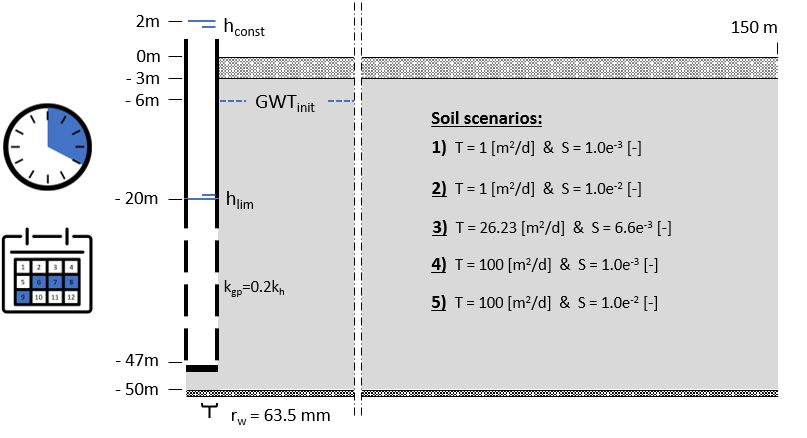
\includegraphics[width=0.7\linewidth]{Schematic_base_model}};  
\node[title, right=10pt] at (box.north west) {Schematic base model definition};
\end{tikzpicture}
\captionsetup{justification=centering}
\caption{Schematic base model definition}
\label{fig:Schematic_base_model}
\end{figure}

\subsection{Well dimensions \& pump placement}
Base model design (not subjected to upscaling) accommodates a single well with a radius of 0.0635 m (2.5 inch). Water displacement between well and aquifer is possible through a partially penetrating screen. Well skin perforation are present from 20 to 47m below model top. It is assumed the, in total 27 m, screen is clean. Due to the tiny nature of wall perforations (and constructional soil improvement around the borehole) a well skin resistance is taken into account. More information on skin resistance is included in Section \ref{section:MODFLOW_const}. Dry season groundwater withdrawal is possible through the installation of a pump. The model contains a pump at an elevation of -30 m. A drop in GWT is preferable limited to an elevation of -20 m (14 m drawdown relative to initial conditions). In this way the occurrence of well screen dry-out and pump malfunctioning is prevented.

\subsection{Time frame} 
ASR-systems can theoretically add value to groundwater availability constantly. Seasonal system behaviour is simulated by a year-round (long term) temporal model resolution. For a duration of four months, starting on June 1$^{st}$, gravity based infiltration simulates wet season flooding. A constant (122 days) 2 m inundation level (on top of well) is assumed (Figure \ref{fig:Schematic_base_model}). In the subsequent eight months of dry season no flooding or rainfall is accounted. Dry season water withdrawal takes place by four hours of pumping daily (243 days). Intermediate day time offers time-space for GWT recovery. \\

Applied conditions serve research purposes. Assumptions made, are not by definition realistic. Actual wet season inundation levels are expected to fluctuate over time. And groundwater withdrawal needs day-specific tuning with respect to agricultural needs. Aspects advisable to take into account in further research. 

\section{MODFLOW model design}
\label{section:MODFLOW_const}
For the ASR-system simulation MODFLOW is used. A finite difference model, written by US Geological Survey (USGS). It is stated to be the worldwide most convenient (open source) computer program for the simulation of groundwater flow. MODFLOW has a modular structure. A variety of aquifer features can be simulated by the introduction of (free available) packages. In this research, input files (needed by MODFLOW) are created by the use of Python and the \texttt{FloPy} package (\citep{Niswonger2011,HarbaughArlen2005}). \\

Unmodified versions of MODFLOW uses Cartesian geometry. Simulations are standard performed in a (single or multi layer) rectangular grid model. These models can simulate the three-dimensional ASR-system performance accurately. However, it requires disadvantageous large computational power. In this particular case the single well simulation is approached axially symmetric. As prescribed by \citet{Langevin2008}, the rectangular model structure is radially scaled by the adjustment of several input parameter. Results are advantageous on model precision and run times. A detailed description of this radial scaled MODFLOW model can be found in Appendix \ref{MODFLOW_radial}. \\

Due to the applied MODFLOW radial scaling the defined grid consist of a single row (1 m width) and multiple columns. The well is located in the first cell (column 0, row 0). Column width increases (grouped) stepwise, based on the (radial) distance between the specific column and the well. By the use of the cell sizes 0.0635 m (40x), 0.1 m (25x), 0.5 m (20x), 1.0 m (25x), 2.0 m (30x) and 5.0 m (10x) a total (radial) length of 150 m is simulated. An extent assumed to be sufficient for the purposes of this research (Appendix \ref{section:Leakage_factor}. The vertical (third) dimension is added to the model by a total of 50 layers (thickness of 1.0 m each). \\

Model timespan (one year) is devised into an abundance of logarithmic time frames. Higher temporal resolutions is added to the moments at which fluctuation in head are expected. The design of four months infiltration contains a single logarithmic time frame of 200 steps. Every single day in dry season (243 days) contains a 4 hour logarithmic time frame for pumping (8 steps) and a subsequent 20 hour logarithmic time frame for recovery (10 steps). This puts the year-round total number of time steps on 4574. 

\subsection{MODFLOW-NWT} 
Due to initial conditions and expected strong temporal variations in GWT cells may fall dry and become wet again over time. Model simulation is therefore performed through the use of MODFLOW-NWT: The Newton-Raphson formulation for the (more convenient) MODFLOW-2005 program. As stated by \citet{Niswonger2011}, MODFLOW-NWT is intended for solving problems involving drying and re-wetting non-linearities of the unconfined groundwater-flow equation. MODFLOW-NWT requirs a combined use with the \texttt{Upstream Weighting (UPW)} package for calculation conductances between cells (instead of the \texttt{BCF}, \texttt{LPF} or \texttt{HUF} package applicable with MODFLOW-2005). The \texttt{UPW} package keeps dry cells active, while water outflow of the cell is not allowed. Moreover, if applicable inflow to a dry cell automatically flows further down to the adjacent (non-dry) cell in the layer below \citep{Niswonger2011}. In correspondence with the use of MODFLOW-NWT the (own) NWT solver is used for model simulation (instead of the convenient \texttt{PCG} solver). 

\subsection{MODFLOW - \texttt{GHB}}
Wet season infiltration is included by the use of the \texttt{General Head Boundary} (\texttt{GHB}) package. For as long as the wet season (stress periods), \texttt{GHB} cells are specified through \texttt{stress period data}. \texttt{General Head Boundaries} are added to the well cells (row 0, column 0) in the predefined layers of penetration (layer 20-46). The \texttt{GHB stress period data} requires an additional definition of \texttt{stage} and \texttt{cond} (conductance) \citep{Harbaugh2000}. The stage equals the constant flood inundation level (h$^*$ = 2 m). For the purposes of this research conductances are aligned with the \texttt{CWC} (Cell-to-Well hydraulic conductance). More information on the \texttt{CWC} can be found in Section \ref{subsec:MODFLOW_MNW2}. 

\subsection{MODFLOW - \texttt{MNW2}}
\label{subsec:MODFLOW_MNW2}
The ASR-system of interest contains a well which is partially penetrating the aquifer. In simulation the aquifer consisting of multiple model layers. A set-up causing the convenient \texttt{Well} package to be insufficient. For a solid simulation the more extended \texttt{Multi-Node-Well2} (\texttt{MNW2}) package is used. \texttt{MNW2} houses several additional well options (e.g. bounded drawdown, addition of well skin resistances and pump related adjustments in discharge). Thence, definition of an abundant list of parameters is required (within \texttt{node data} and \texttt{stress period data})\citep{LeonardF.KonikowGeorgeZ.HornbergerKeithJ.Halford2009}.  \\

Many parameters are default correct, some however need specification. The well penetration interval (screen) is recorded by the definition of \texttt{ztop} and \texttt{zbotm}. \texttt{MNW2} assigns the well screen to model nodes (well cells in the corresponding layers). In-well GWT preferable does not drop below the elevation of -20 m. \texttt{Hlim} definition guarantees this desire. The flag of \texttt{qlimit} is 1 activates the definition of \texttt{Hlim}. Moments (stress-periods) of pump operation are set by \texttt{ITMP} is 1, all other moments (stress-periods) \texttt{ITMP} is set 0. Furthermore, \texttt{MNW2} requires the input of a desired discharge (\texttt{qdes} and specification of Cell-to-Well hydraulic conductance (\texttt{CWC}), topics highlighted below. \\

\textbf{Desired discharge (\texttt{qdes})} \\
Based on a predefined desired discharge the MNW2 determines a (model) layer dependent discharge iteratively. As long as the head bound (\texttt{Hlim}) is not restrictive, summed layer discharges equal (approximately) the desired discharge. Desired discharges are based on the analytical Thiem method \citep{Kruseman2000}; confined steady state flow equation \ref{eq:Q_thiem}: \\

\begin{equation}
 Q_{Thiem} = \frac{2\pi KD (s_{well}- s_{2})}{ln(r_{2}/r_{well})}
\label{eq:Q_thiem}
\end{equation}  

where $Q_{Thiem}$ (m$^3$/d) is the confined steady state well discharge, $K$ (m/d) is the aquifer hydraulic conductivity, D (m) is aquifer height, $s_{well}$ (m) the in-well drawdown, $s_{2}$ (m) is the drawdown at a known second location, $r_{2}$ (m) is the distance between the second location and the well and $r_{well}$ (m) equals the well radius. \\

In this particular case thickness $D$ is interpreted as being the well screen height. And the in-well drawdown is set in correspondence with the desired limit in GWT; $s_{well}$ equals 14 m. Due to different horizontal hydraulic conductivities $K$, obtained desired discharges are scenario dependent. Note, upscaling by borehole cleaning (Section \ref{subsec:Up_clean}) will result in a variation of desired discharges due to the change in screen height ($D$). \\

\texttt{FloPy} is used for reading MODFLOW binary output files. In other words, the actual simulated discharges (and recharges) are obtained by reading the \texttt{binaryfile.CellBudgetFile}. \\

\textbf{Cell-to-Well hydraulic conductance (\texttt{CWC})} \\
Due to \texttt{MNW2} application the occurrence of a difference between the head in the well an d the head in the model (well)cell is inevitable. Multiple model elements contribute to a difference in head. Total head difference is dependent on the expression of Cell-to-Well hydraulic conductance (\texttt{CWC}), depicted in Equation \ref{eq:CWC_n} \citep{LeonardF.KonikowGeorgeZ.HornbergerKeithJ.Halford2009}. 

\begin{equation}
 CWC_n = [A + B + CQ_{n}^{(P-1)}]^{-1}
\label{eq:CWC_n}
\end{equation}  

Where $CWC_n$ (m$^2$/d is the n$^th$ Cell-to-Well hydraulic conductance, A is the linear aquifer-loss coefficient resulting from the well having a smaller radius than the horizontal dimensions of the cell in which it is located, B is the linear well-loss coefficient accounting for head losses that occur adjacent to and within the borehole and well screen (skin effects) and $CQ_{n}^{(P)}$ accounts for non-linear head losses due to turbulent flow near the well \citep{LeonardF.KonikowGeorgeZ.HornbergerKeithJ.Halford2009}. \\

\begin{equation}
 A = \frac{ln(r_{o}/r_{w})}{2\pi b \sqrt{K_{x}K_{y}}}
\label{eq:A}
\end{equation}

\begin{equation}
 r_o = 0.14 \sqrt{\Delta x^2 + \Delta y^2}
\label{eq:r_o}
\end{equation}

\begin{equation}
 B = \frac{SKIN}{2\pi b \sqrt{K_{x}K_{y}}}
\label{eq:B}
\end{equation}   

\begin{equation}
 SKIN = {(\frac{bK_{h}}{b_{w}K_{SKIN}}-1)} ln(\frac{r_{skin}}{r_{w}})
\label{eq:SKIN}
\end{equation}   

Where $r_{o}$ (m) is the effective external radius of a rectangular finite-difference cell for isotropic porous media, $r_{w}$ (m) is the well radius, $r_{skin}$ (m) is the well radius plus the thickness of improved soil around the well, b (m) is the saturated thickness of the cell(layer), $b_{w}$ (m) is the saturated (active) length of the borehole in the cell(layer) (in the purposes of this research equal to b (1m)), $K_{h}$ (m/d) is the horizontal (non-radial scaled) hydraulic conductivity (equals $K_{x}$ and $K_{y}$ due to the assumption of horizontal anisotropy), $\Delta x$ (m) is the grid spacing in the x-(column-)direction and $\Delta y$ (m) is the grid spacing in the y-(row-)direction \citep{LeonardF.KonikowGeorgeZ.HornbergerKeithJ.Halford2009}. \\

As stated, the aquifer-loss coefficient (A) accounts for the difference in dimensions between the well (cross-section) and the (well)cell. Perfectly understandable in the case of an unmodified (Cartesian geometry) rectangular grid MODFLOW model. Simulation in this research is however performed in a radial scaled model, according to the principles as stated by \citet{Langevin2008}. Well cell width perfectly aligns the radius of the well. Therefore it is assumed the A term is negligible. In addition, laminar (non-turbulent) flow is expected near the well (ignorance of $CQ_{n}^{(P)}$ term). Further research should substantiate or refute these assumptions. \\

What left, is a \texttt{CWC} dependent on the well-loss coefficient B. In the SKIN term (part of coefficient B) the parameters $r_{skin}$ and $K_{skin}$ need additional information. $r_{skin}$, equals $r_{w}$ plus a unknown radius of improved soil around the well. As stated by \citep{Bot2016}, for proper installation a minimum length of 0,125 m (measured from well radius) is required. This length is therefore implemented in research. $K_{skin}$ accounts for both; a higher resistance due to the well screen tiny perforations and at the same time a reduction in resistance due to the improved soil around the well. Further research should be applied to get deeper understanding of the exact parameter magnitude. $K_{skin}$ is typically expected to be lower than the $K_{h}$ \citep{LeonardF.KonikowGeorgeZ.HornbergerKeithJ.Halford2009}. Dependent on the scenarios three different values are assumed in research, as depicted in Figure \ref{fig:Schematic_base_model}. Resulting \texttt{CWC} values used in the different base models are; 0.031 m$^2$/d (sc1\&2), 0.358 m$^2$/d (sc3) and 0.512 m$^2$/d (sc4\&5). Note, upscaling the borehole cross-sectional dimension (Section \ref{Subsec:Up_diam}) will result in variation of \texttt{CWC} values due to the change in $r_{w}$ and thus $r_{skin}$. 

\section{Base model performance}
\label{section:Base_model_perf}
On the base of the different soil scenarios (Figure \ref{fig:Schematic_base_model}) the performances of five base models are taken into account. In terms of time (within the model year) a division can be made between the wet and dry season. Wet season ASR-system behaviour is characterized by the inflow of water. Analysis is pointed at the volumes recharged and the impact of these volumes on GWT. In the subsequent eight months of drought, the system works in reverse. In this time of year, maximum pump operation and the accompanied impact on GWT is of key interest. As supplement the mutual relation between in- and outflow is considered. This is done by the introduction of the recovery ratio (Equation \ref{eq:RR}). Through this term the system impact on nature is discussed.  

\begin{equation}
 R_{\%} = \frac{V_{out,tot}}{V_{in,tot}}
\label{eq:RR}
\end{equation}

Where  R$_{\%}$ is the year-round recovery ratio (-), $V_{in,tot}$ (m$^3$) is the wet season total volume recharged and $V_{out,tot}$ (m$^3$) is the dry season total volume discharged. $R_{\%}$ values smaller than 1 (-) suggests a sustainable system interaction with nature.  \\

\textbf{Wet season behaviour} \\
Recharge due to flooding has a slightly above average start. After a few days the inflow reaches an equilibrium. From this moment onwards water accumulates in the aquifer at an approximately constant rate. This course takes place in all scenarios. Order of volume do differ and increases in correspondence with the scenarios. The example scenario 3 cross-sectional contour (Figure \ref{fig:Example_Sc3_base_cont_wet}), visualizes the system behaviour at the begin (day 5) and absolute end of wet season (day 122).

\begin{figure}[h!]
	\centering
	\begin{subfigure}[b]{0.5\linewidth}
		\centering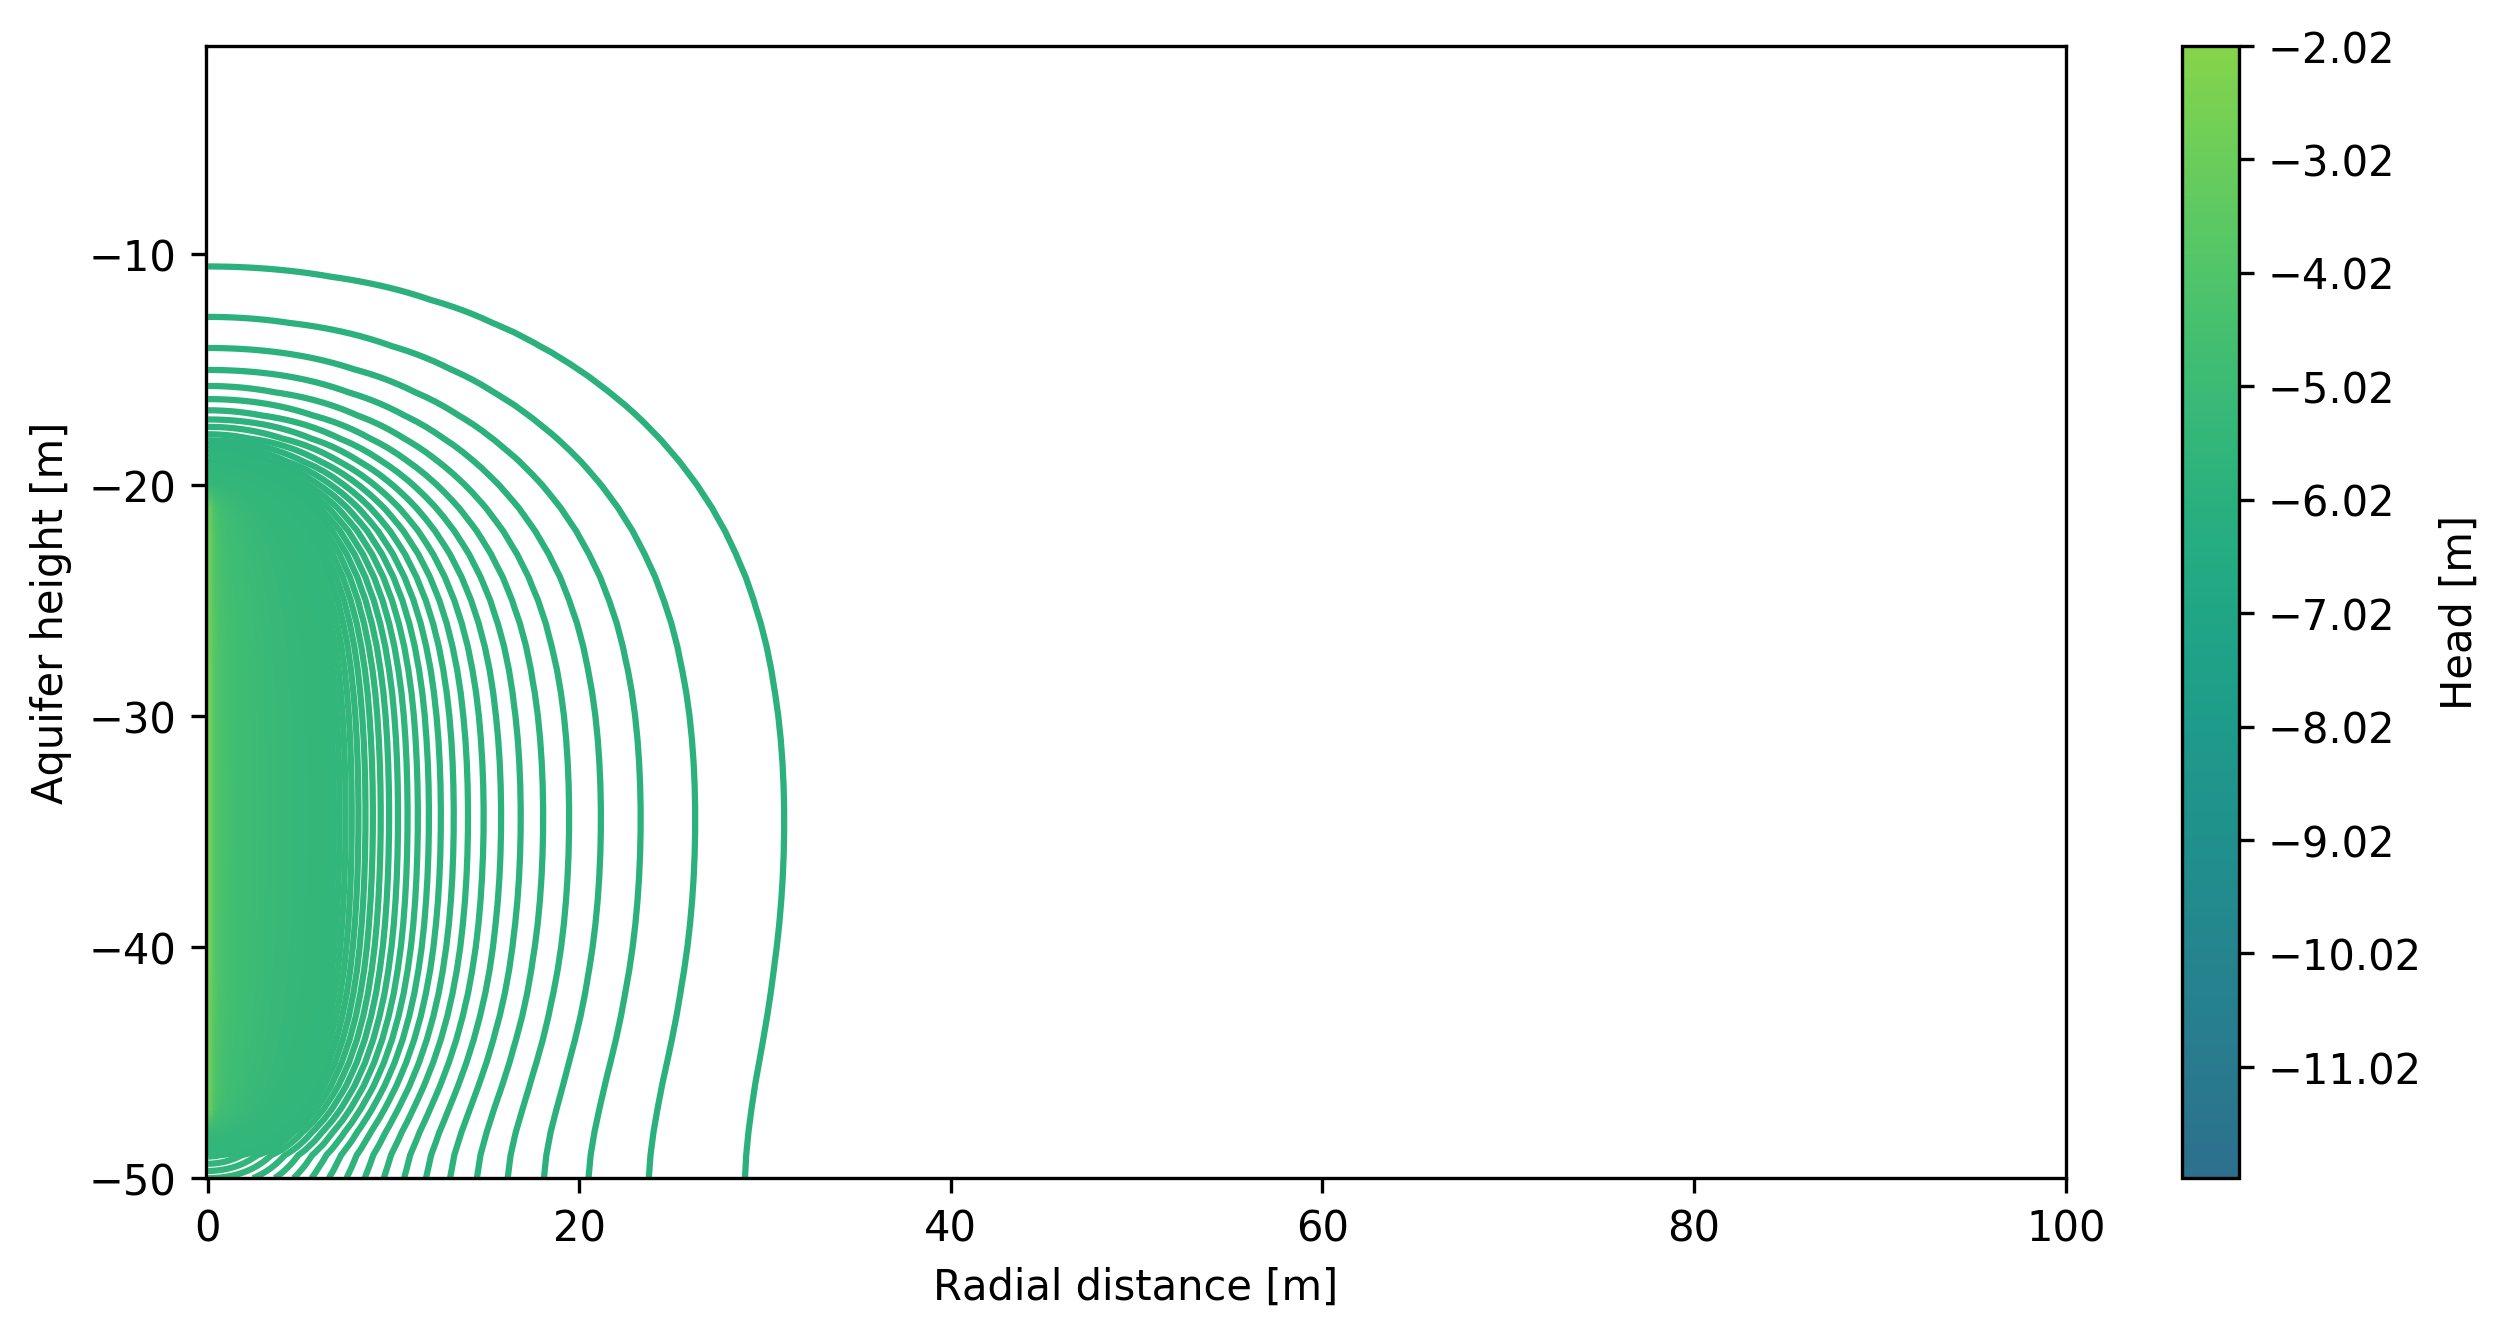
\includegraphics[width=\linewidth]{Sc3a1_cont_d5}
		\captionsetup{justification=centering}		
		\caption{\label{fig:Sc3a1_cont_d5}}
		\end{subfigure}\hfill
	\begin{subfigure}[b]{0.5\linewidth}
        \centering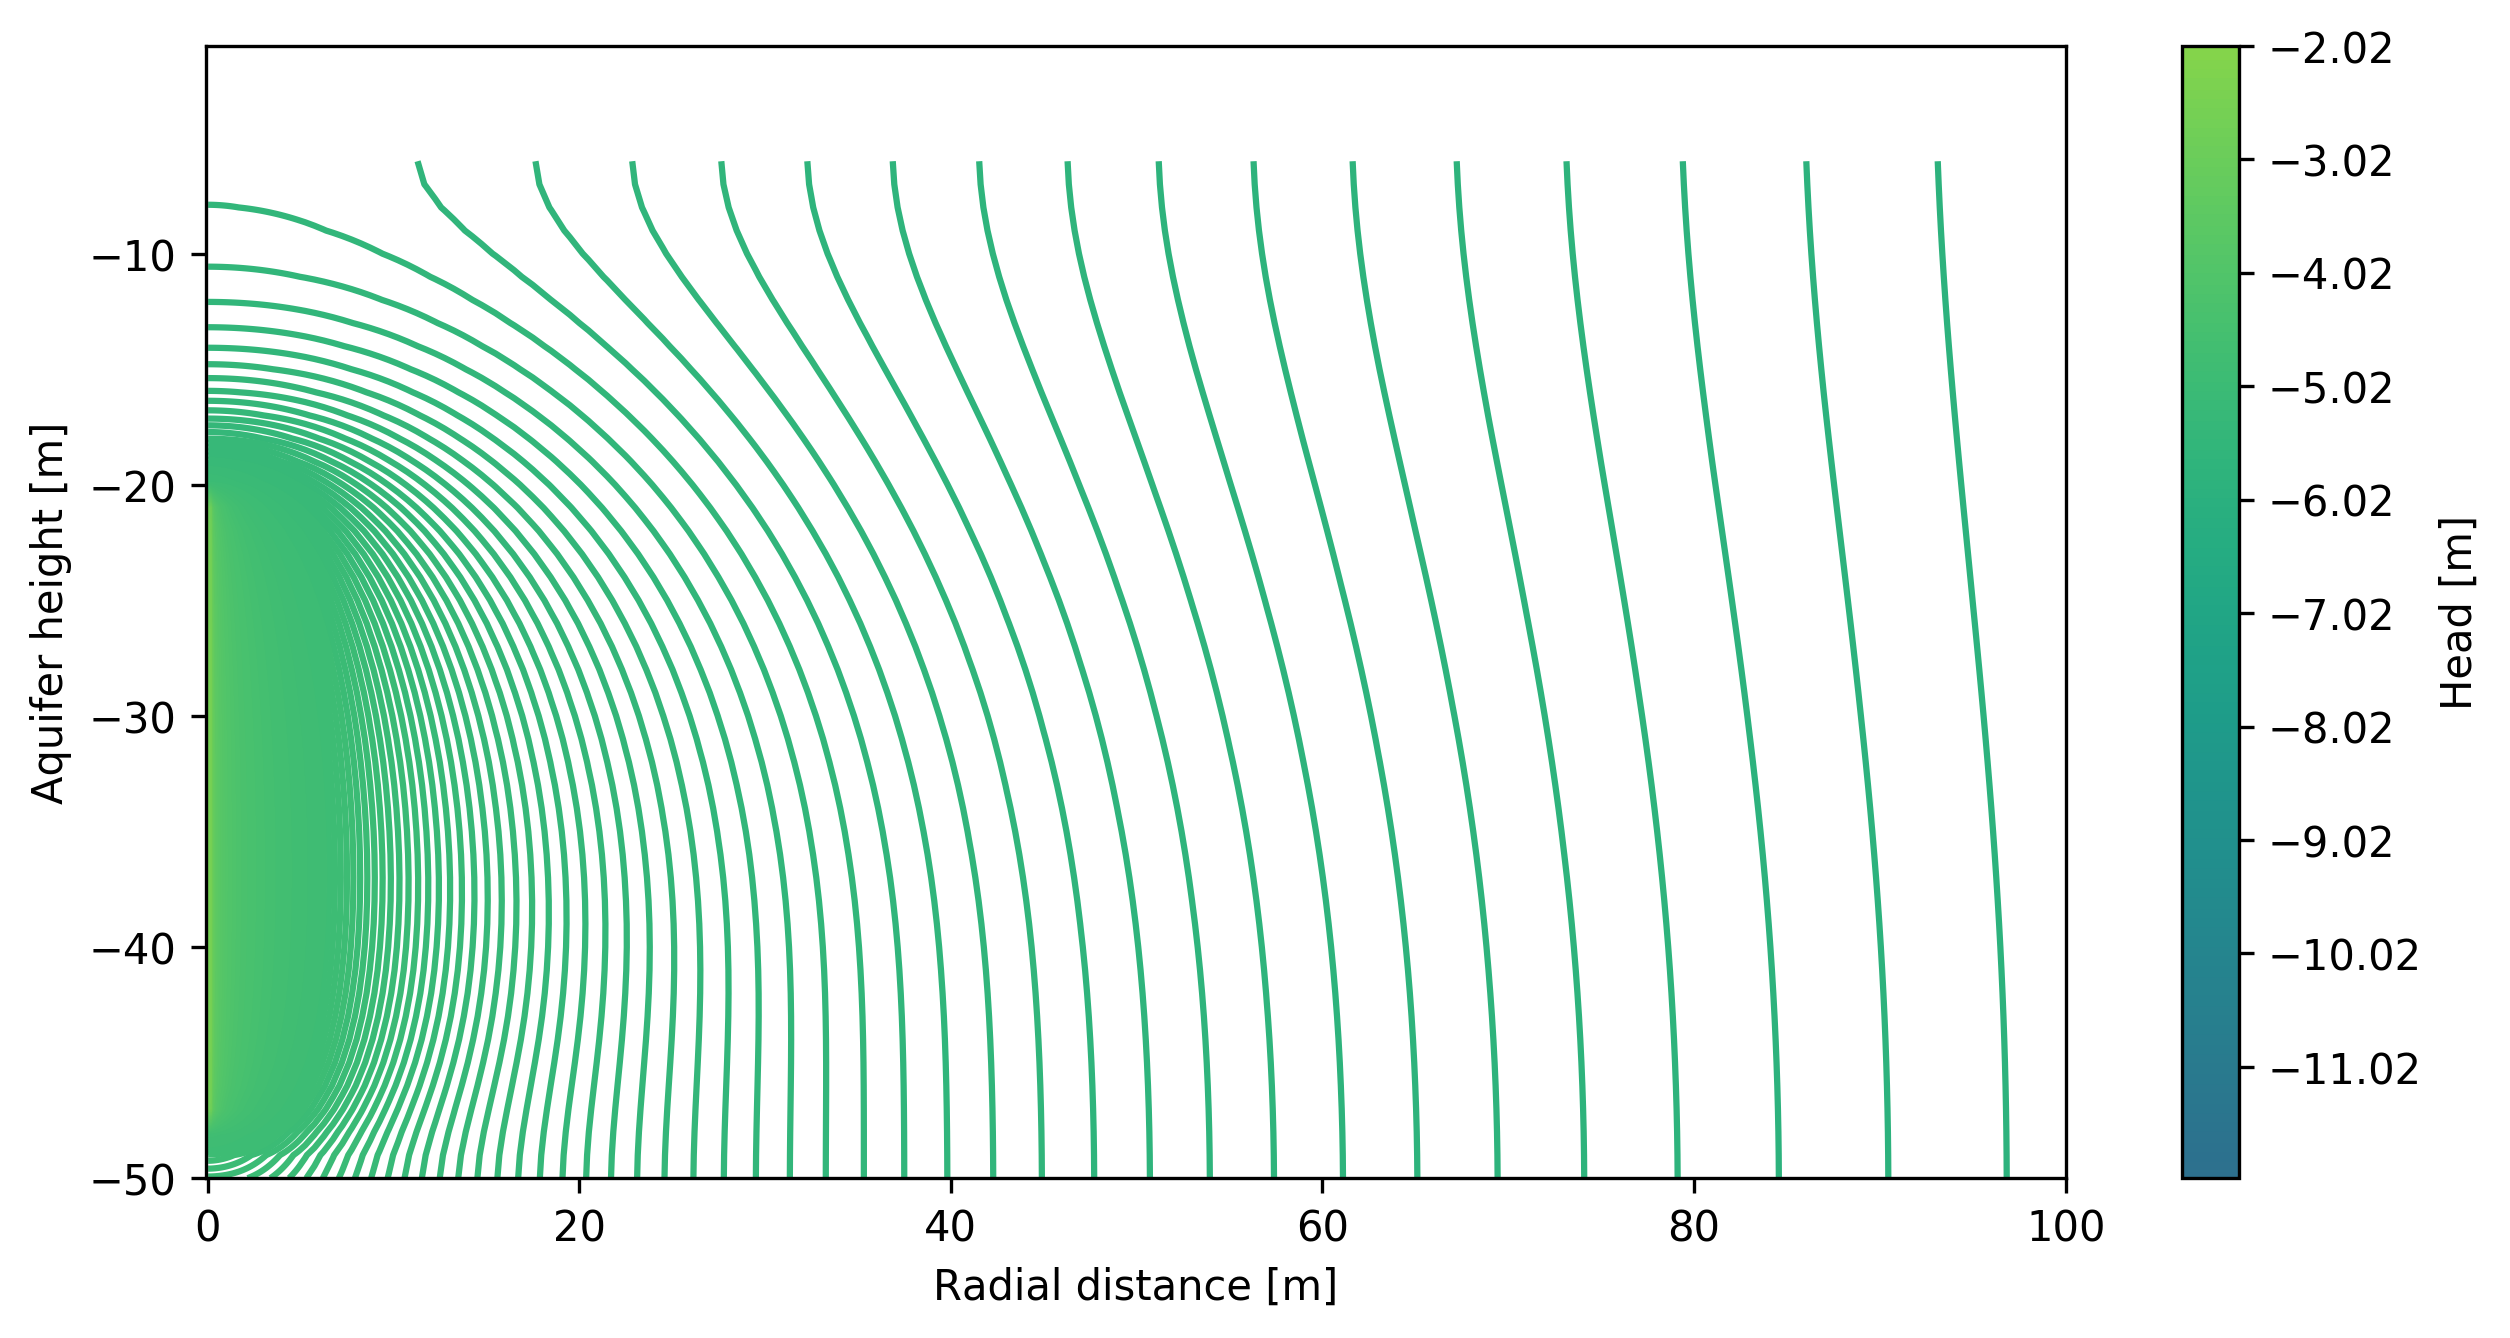
\includegraphics[width=\linewidth]{Sc3a1_cont_d122}
		\captionsetup{justification=centering}		
		\caption{\label{fig:Sc3a1_cont_d122}}
		\end{subfigure}
		\captionsetup{justification=centering}	
	\caption{Example scenario 3 - base model - Cross-sectional contour head after (\subref{fig:Sc3a1_cont_d5}) five days and (\subref{fig:Sc3a1_cont_d122}) 122 days of infiltration} 
	\label{fig:Example_Sc3_base_cont_wet}
\end{figure} 

Impacts on the groundwater table are also dominant at simulation front. At close well range relative large increases in groundwater heads are encountered in the first days. These heads do not reach the predefined flood level, not even at the end of wet season. A development justifiable by the implemented well skin resistances. Figure \ref{fig:Example_Sc3_base_head_wet} illustrates the precise impact of flood based ASR-system infiltration on groundwater heads in several representative (model) layers of soil scenario 3. Worth mentioning, groundwater level increase is already limited at a relative short radial distance (steep groundwater cone). Even after 122 days of infiltration the head increase at a radial distances of about 60-80 m is not quite substantial, unregarded the scenario.  

\begin{figure}[h!]
	\centering
	\begin{subfigure}[b]{0.5\linewidth}
		\centering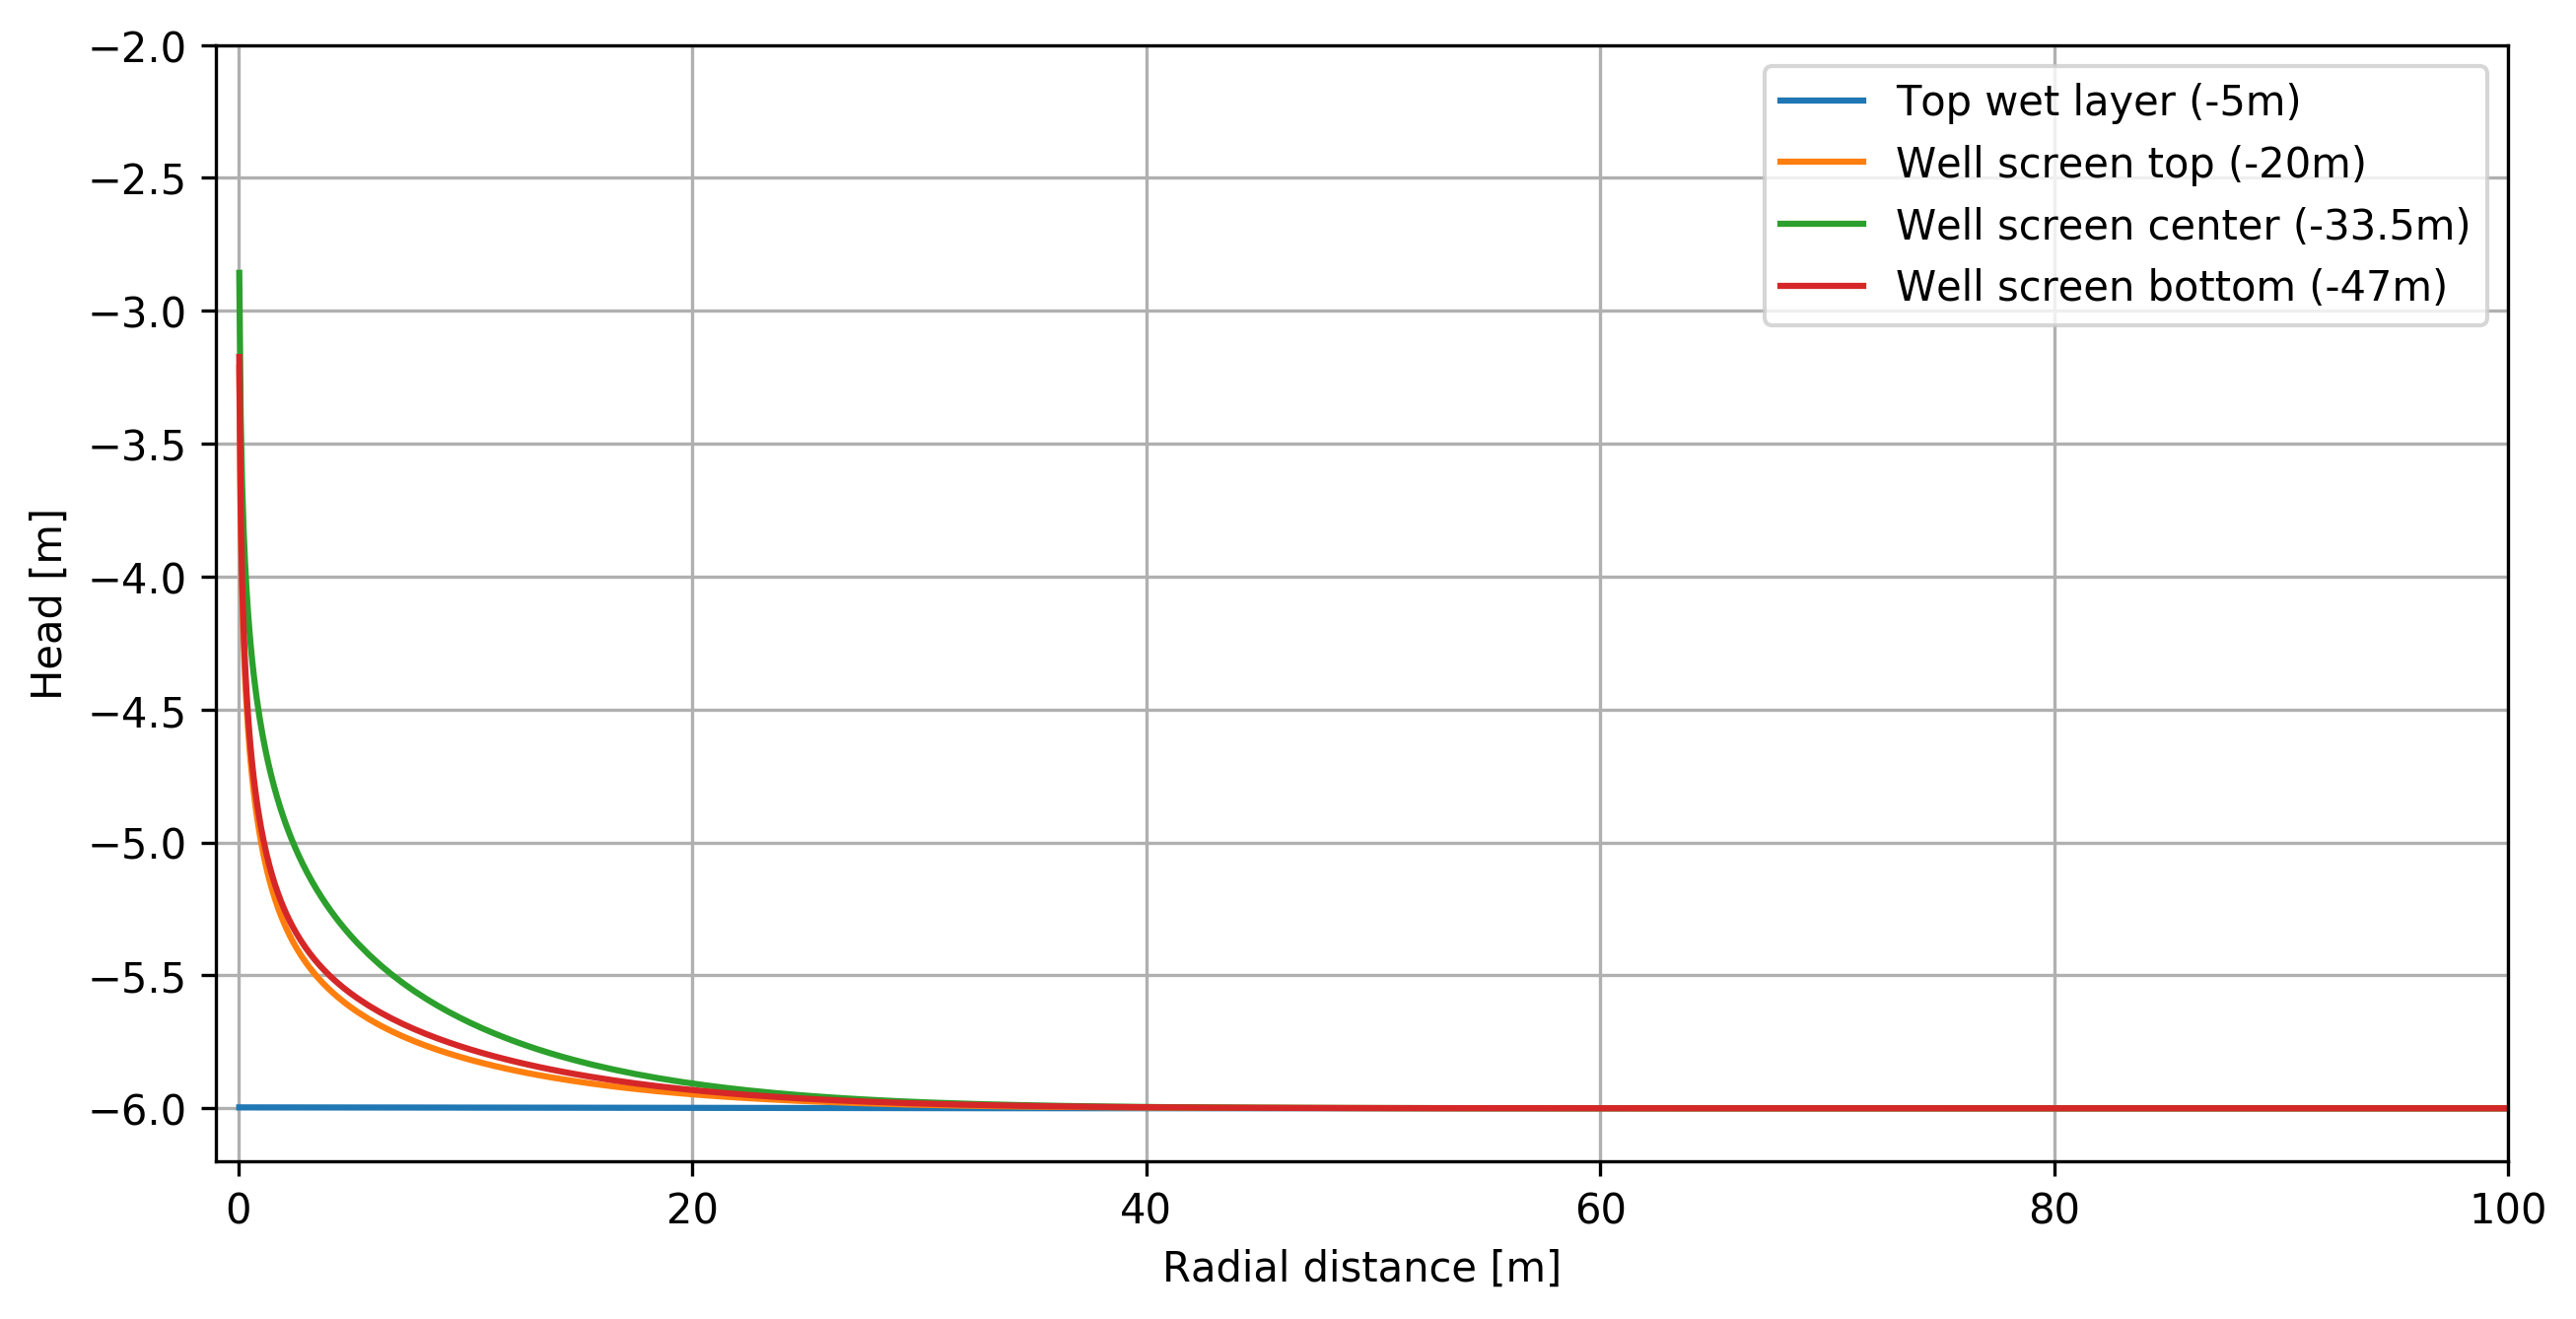
\includegraphics[width=\linewidth]{Sc3a1_head_d5}
		\captionsetup{justification=centering}		
		\caption{\label{fig:Sc3a1_head_d5}}
		\end{subfigure}\hfill
	\begin{subfigure}[b]{0.5\linewidth}
        \centering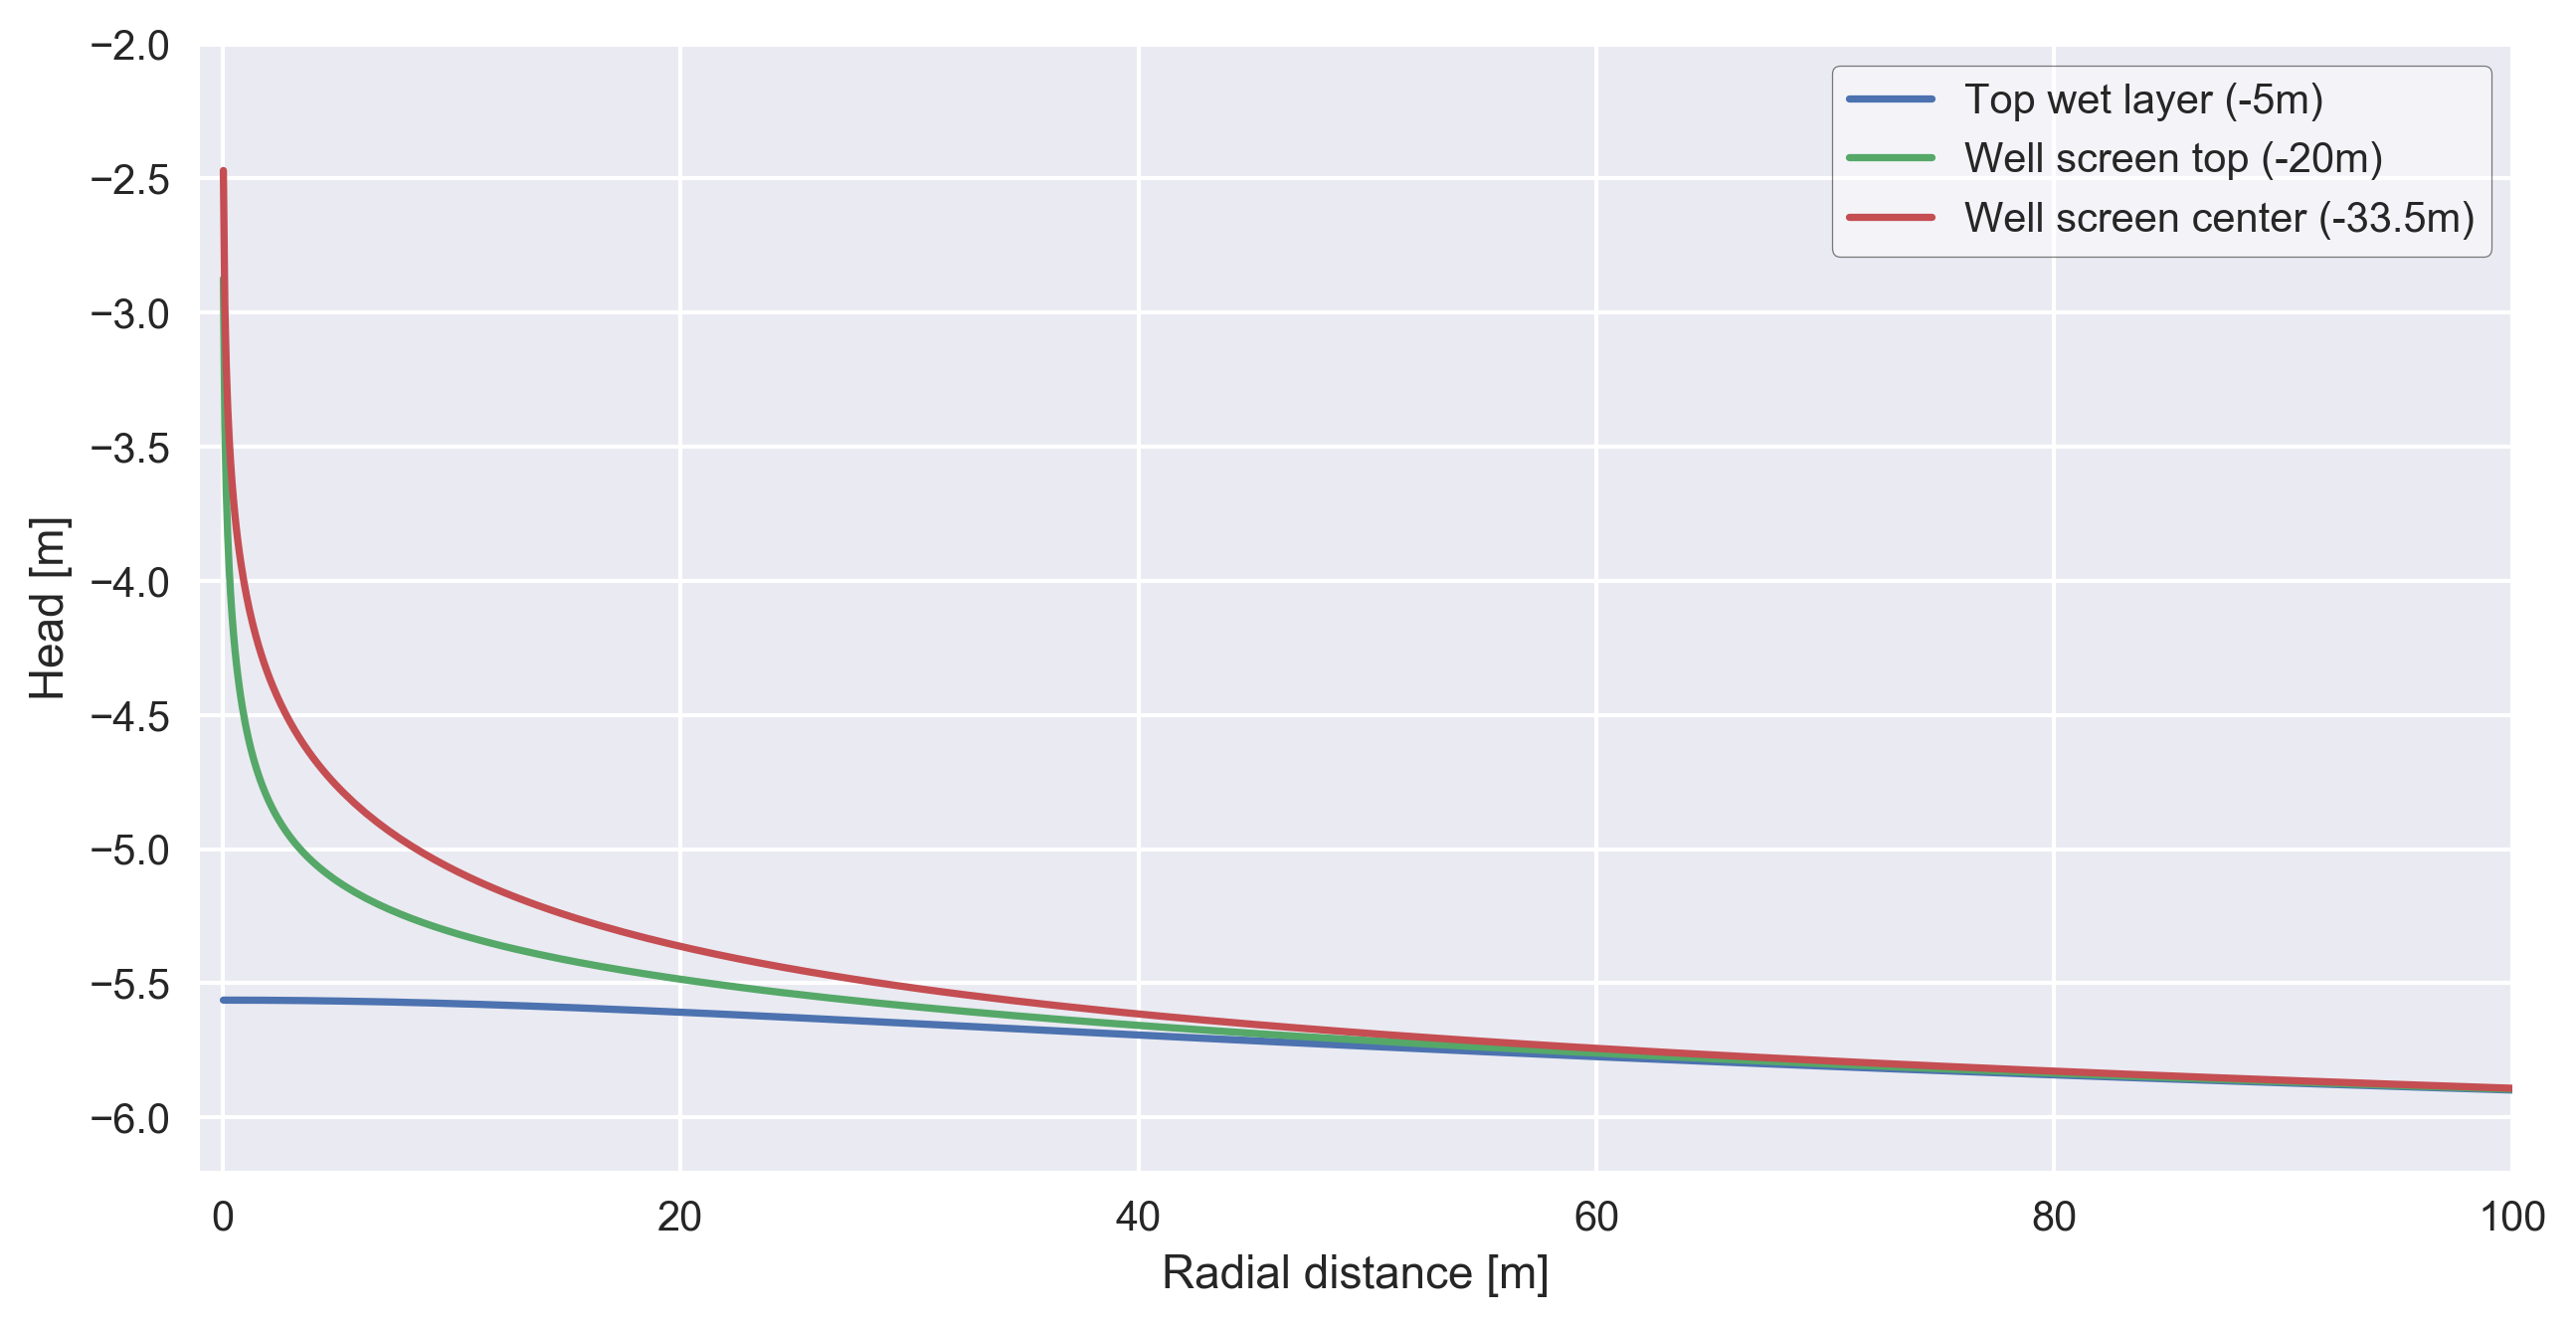
\includegraphics[width=\linewidth]{Sc3a1_head_d122}
		\captionsetup{justification=centering}		
		\caption{\label{fig:Sc3a1_head_d122}}
		\end{subfigure}
		\captionsetup{justification=centering}	
	\caption{Example scenario 3 - base model - Head in representative layers after (\subref{fig:Sc3a1_head_d5}) five days and (\subref{fig:Sc3a1_head_d122}) 122 days of infiltration} 
	\label{fig:Example_Sc3_base_head_wet}
\end{figure} 

Scenario dependent results on total wet season volume inflow are included in Table \ref{tab:Base_recharge}. Differences between scenario 1 and 2 as well as scenario 4 and 5 are small. These scenarios only differ from each other in applied storativity (S). Bandwidth defined variance in storativity appears to have only a limited influence on the inflow of water. Most definitely during the application of higher transmisivities these differences in storativity are negligible.   

\begin{table}[h!]
\small
\centering
\caption{Base model scenarios - Wet season recharge (m3)}
\label{tab:Base_recharge}
\begin{tabular}{l|r|r|r|r|r}
\hline 
\textbf{}               & \textbf{Sc 1} & \textbf{Sc 2} & \textbf{Sc 3} & \textbf{Sc 4}  & \textbf{Sc 5} \\ \hline \hline
Volume in (m$^3$)       & 306.83        & 309.28        & 5373.03       & 10483.17       & 10483.86          \\ \hline    
\end{tabular}
\end{table}

\textbf{Dry season behaviour} \\
Model well discharge originates by a predefined desired discharge ($Q_{thiem}$). In all base model scenarios the desired discharge is not reached (visualized for scenario 3 in Figure \ref{fig:Example_Sc3_base_discharge}). The development can be attributed to the specification of a bound in drawdown. Discharge rates are limited by the head bound (-20 m). At pump operation start, the drop in head reached the bound almost instantaneously. In the subsequent hours of pumping (within day) the head bound keeps decisive. The simulation compensates by a decrease in discharge over time. In practice pumping takes place at a more or less constant rate. It suggests model outcome overestimates the discharged volumes slightly. Mutual comparison between the days shows a difference in total discharge between the first and all other days of pumping. The first day of pumping generates somewhat higher volumes. In the subsequent days discharge is by approximation equal. \\

\begin{figure}[H]
	\centering
	\begin{subfigure}[b]{0.5\linewidth}
		\centering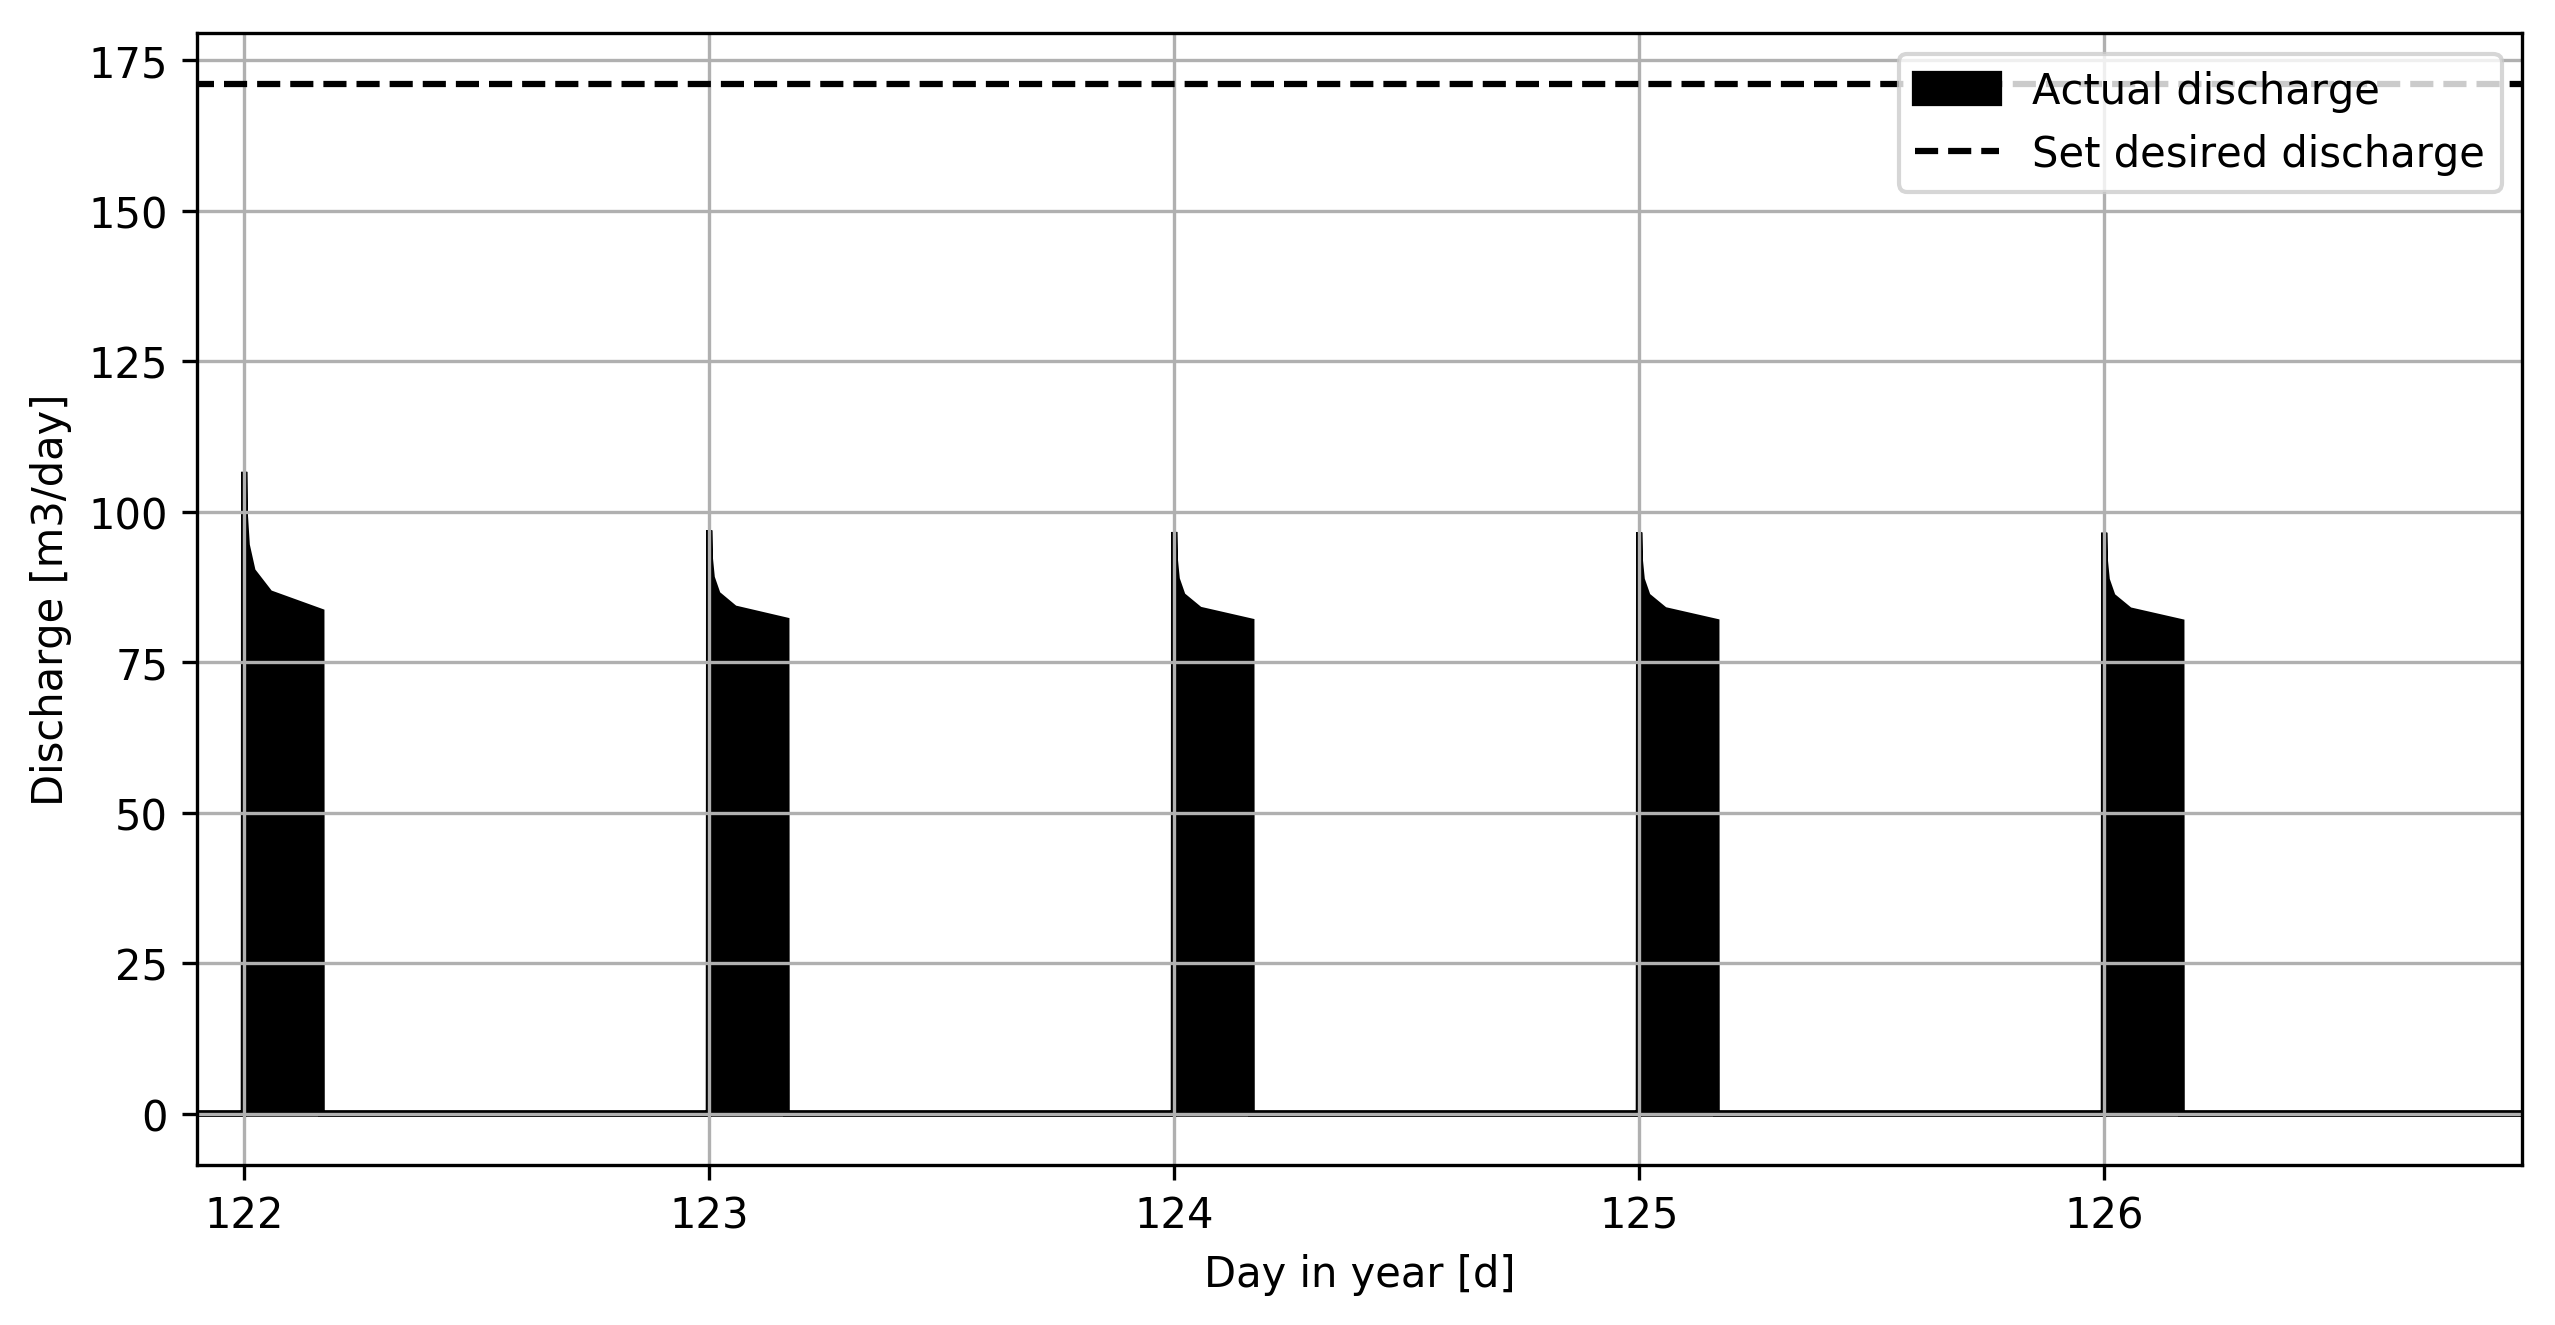
\includegraphics[width=\linewidth]{Sc3a1_Q122_126}
		\captionsetup{justification=centering}		
		\caption{\label{fig:Sc3a1_Q122_126}}
		\end{subfigure}\hfill
	\begin{subfigure}[b]{0.5\linewidth}
        \centering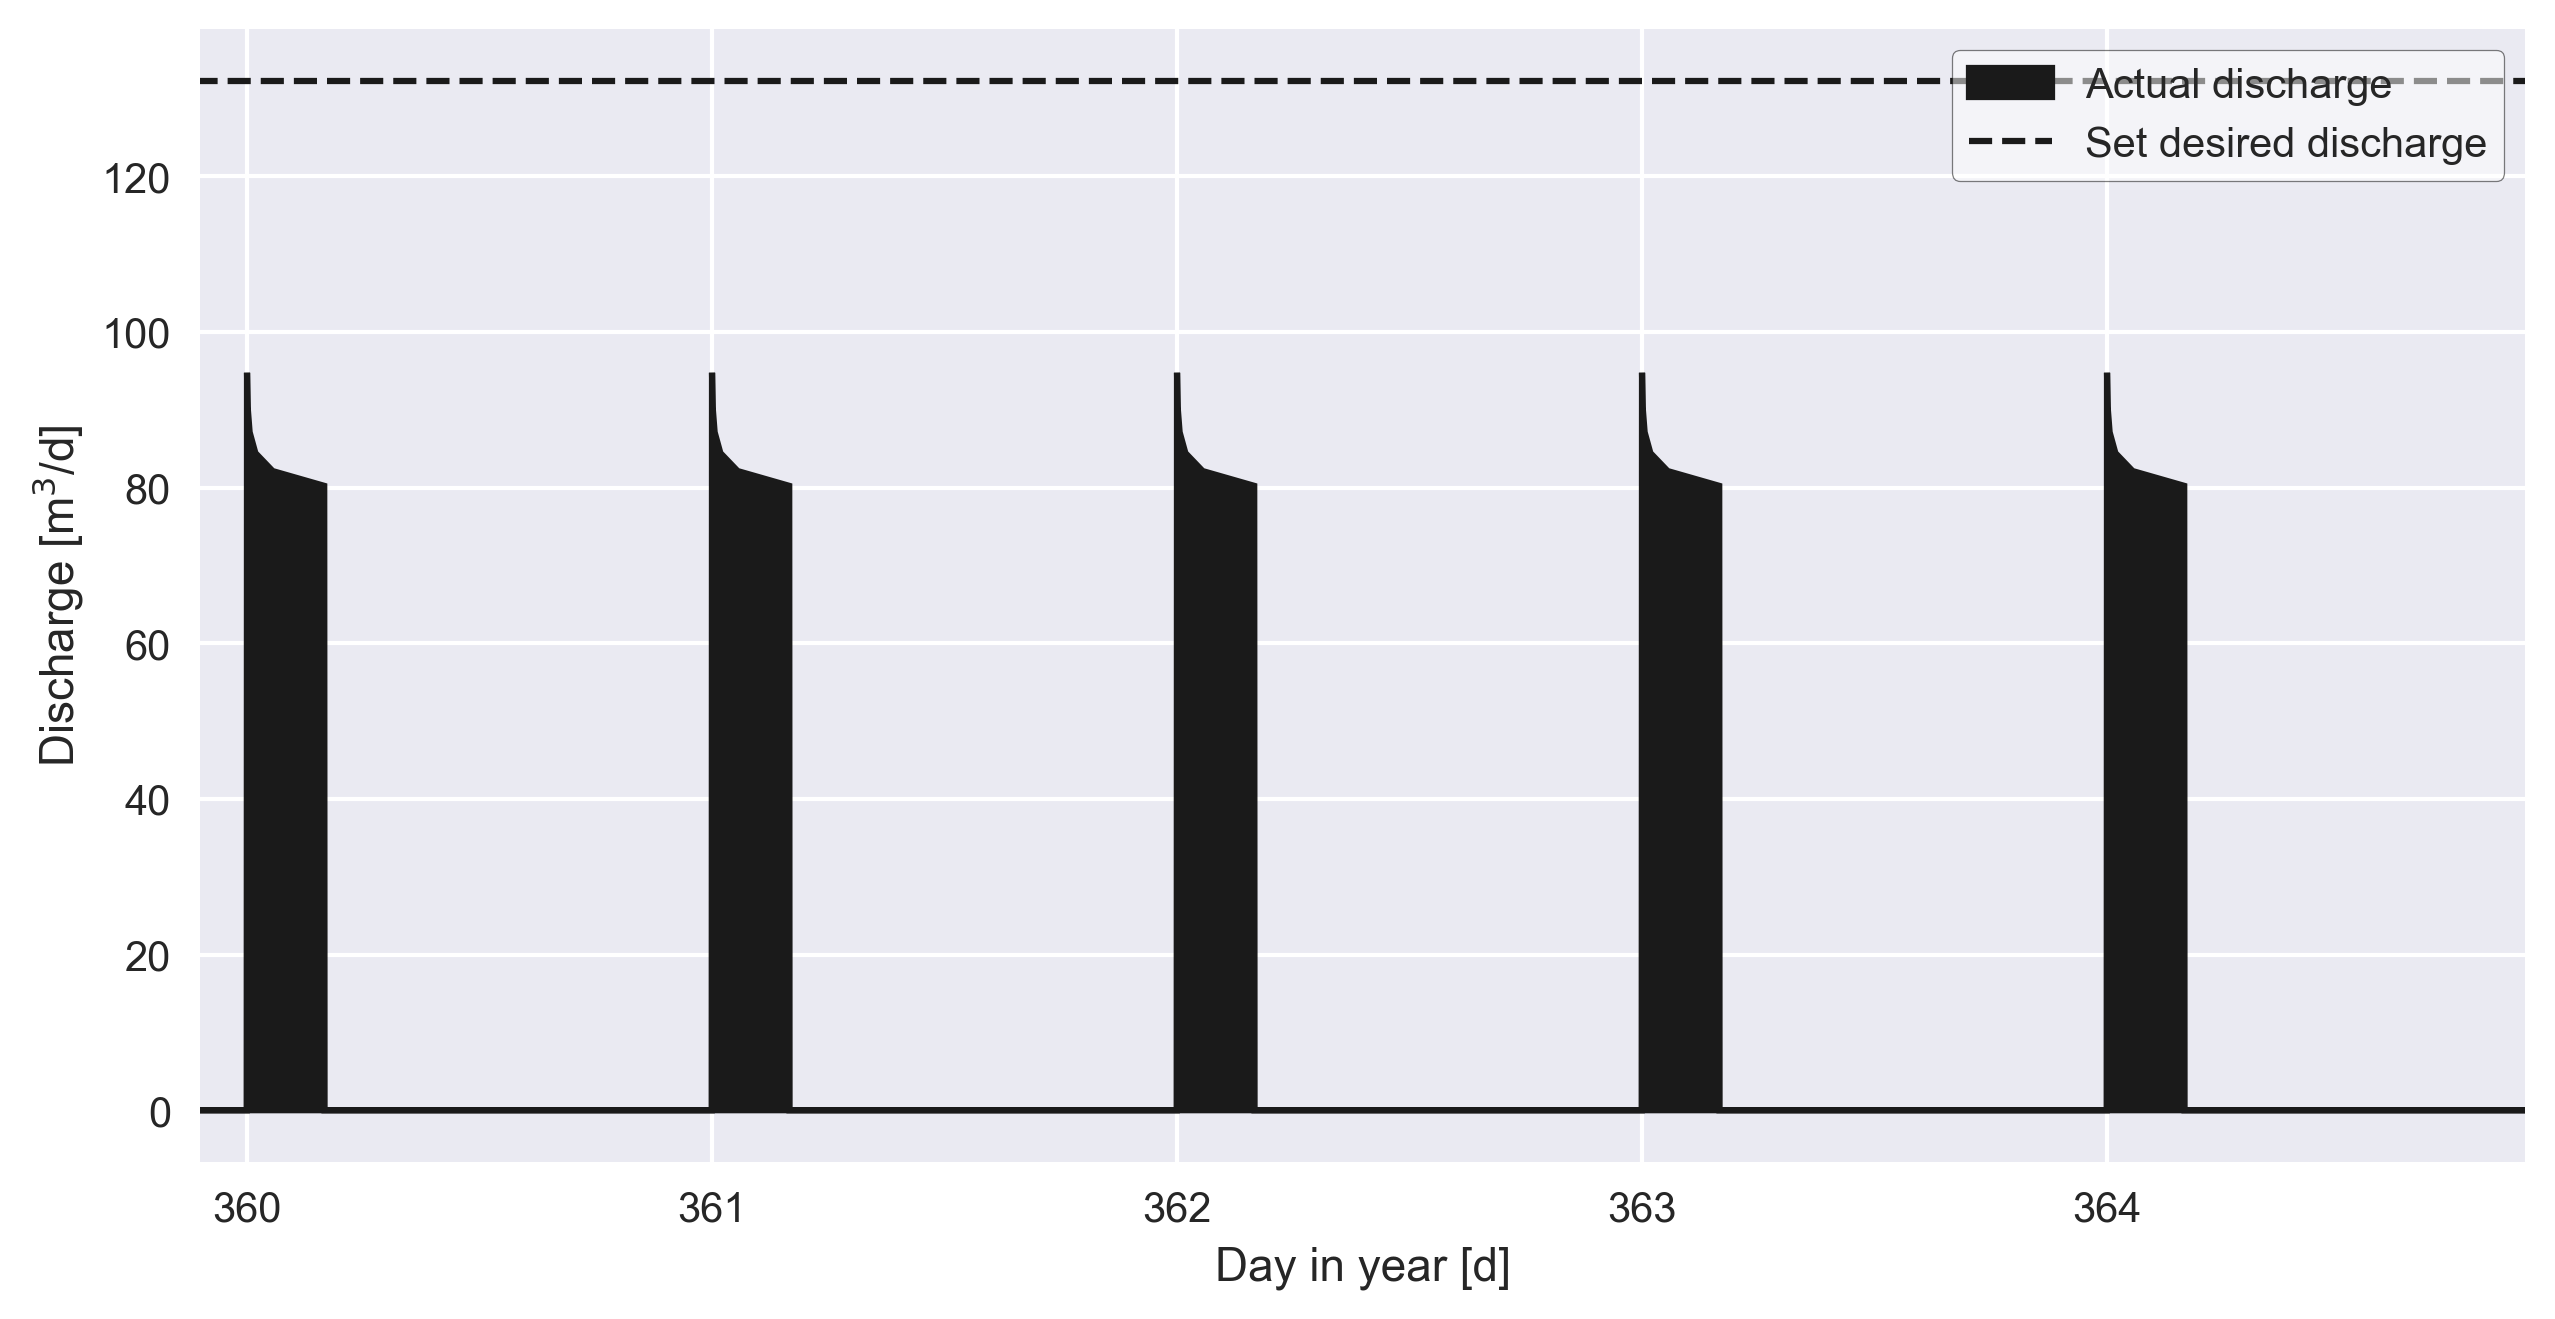
\includegraphics[width=\linewidth]{Sc3a1_Q360_364}
		\captionsetup{justification=centering}		
		\caption{\label{fig:Sc3a1_Q360_364}}
		\end{subfigure}
		\captionsetup{justification=centering}	
	\caption{Example scenario 3 - base model - Discharge performance for   (\subref{fig:Sc3a1_Q122_126}) the first five days and (\subref{fig:Sc3a1_Q360_364}) the last five days of dry season} 
	\label{fig:Example_Sc3_base_discharge}
\end{figure} 

% dit onderstaande plaatje (van bovenstaande 2 in 1 krijg ik via python niet opgeslagen 

%\begin{figure}[h!]
% \centering
% \includegraphics[width=1.0\linewidth]{Sc3a1_Q}
% \captionsetup{justification=centering} 
% \caption{Example on scenario 3 - base model  - discharge performance - for the first and last five days of pumping}
% \label{fig:Example_Sc3_base_dis}
%\end{figure}

\begin{figure}[h!]
	\centering
	\begin{subfigure}[b]{0.5\linewidth}
		\centering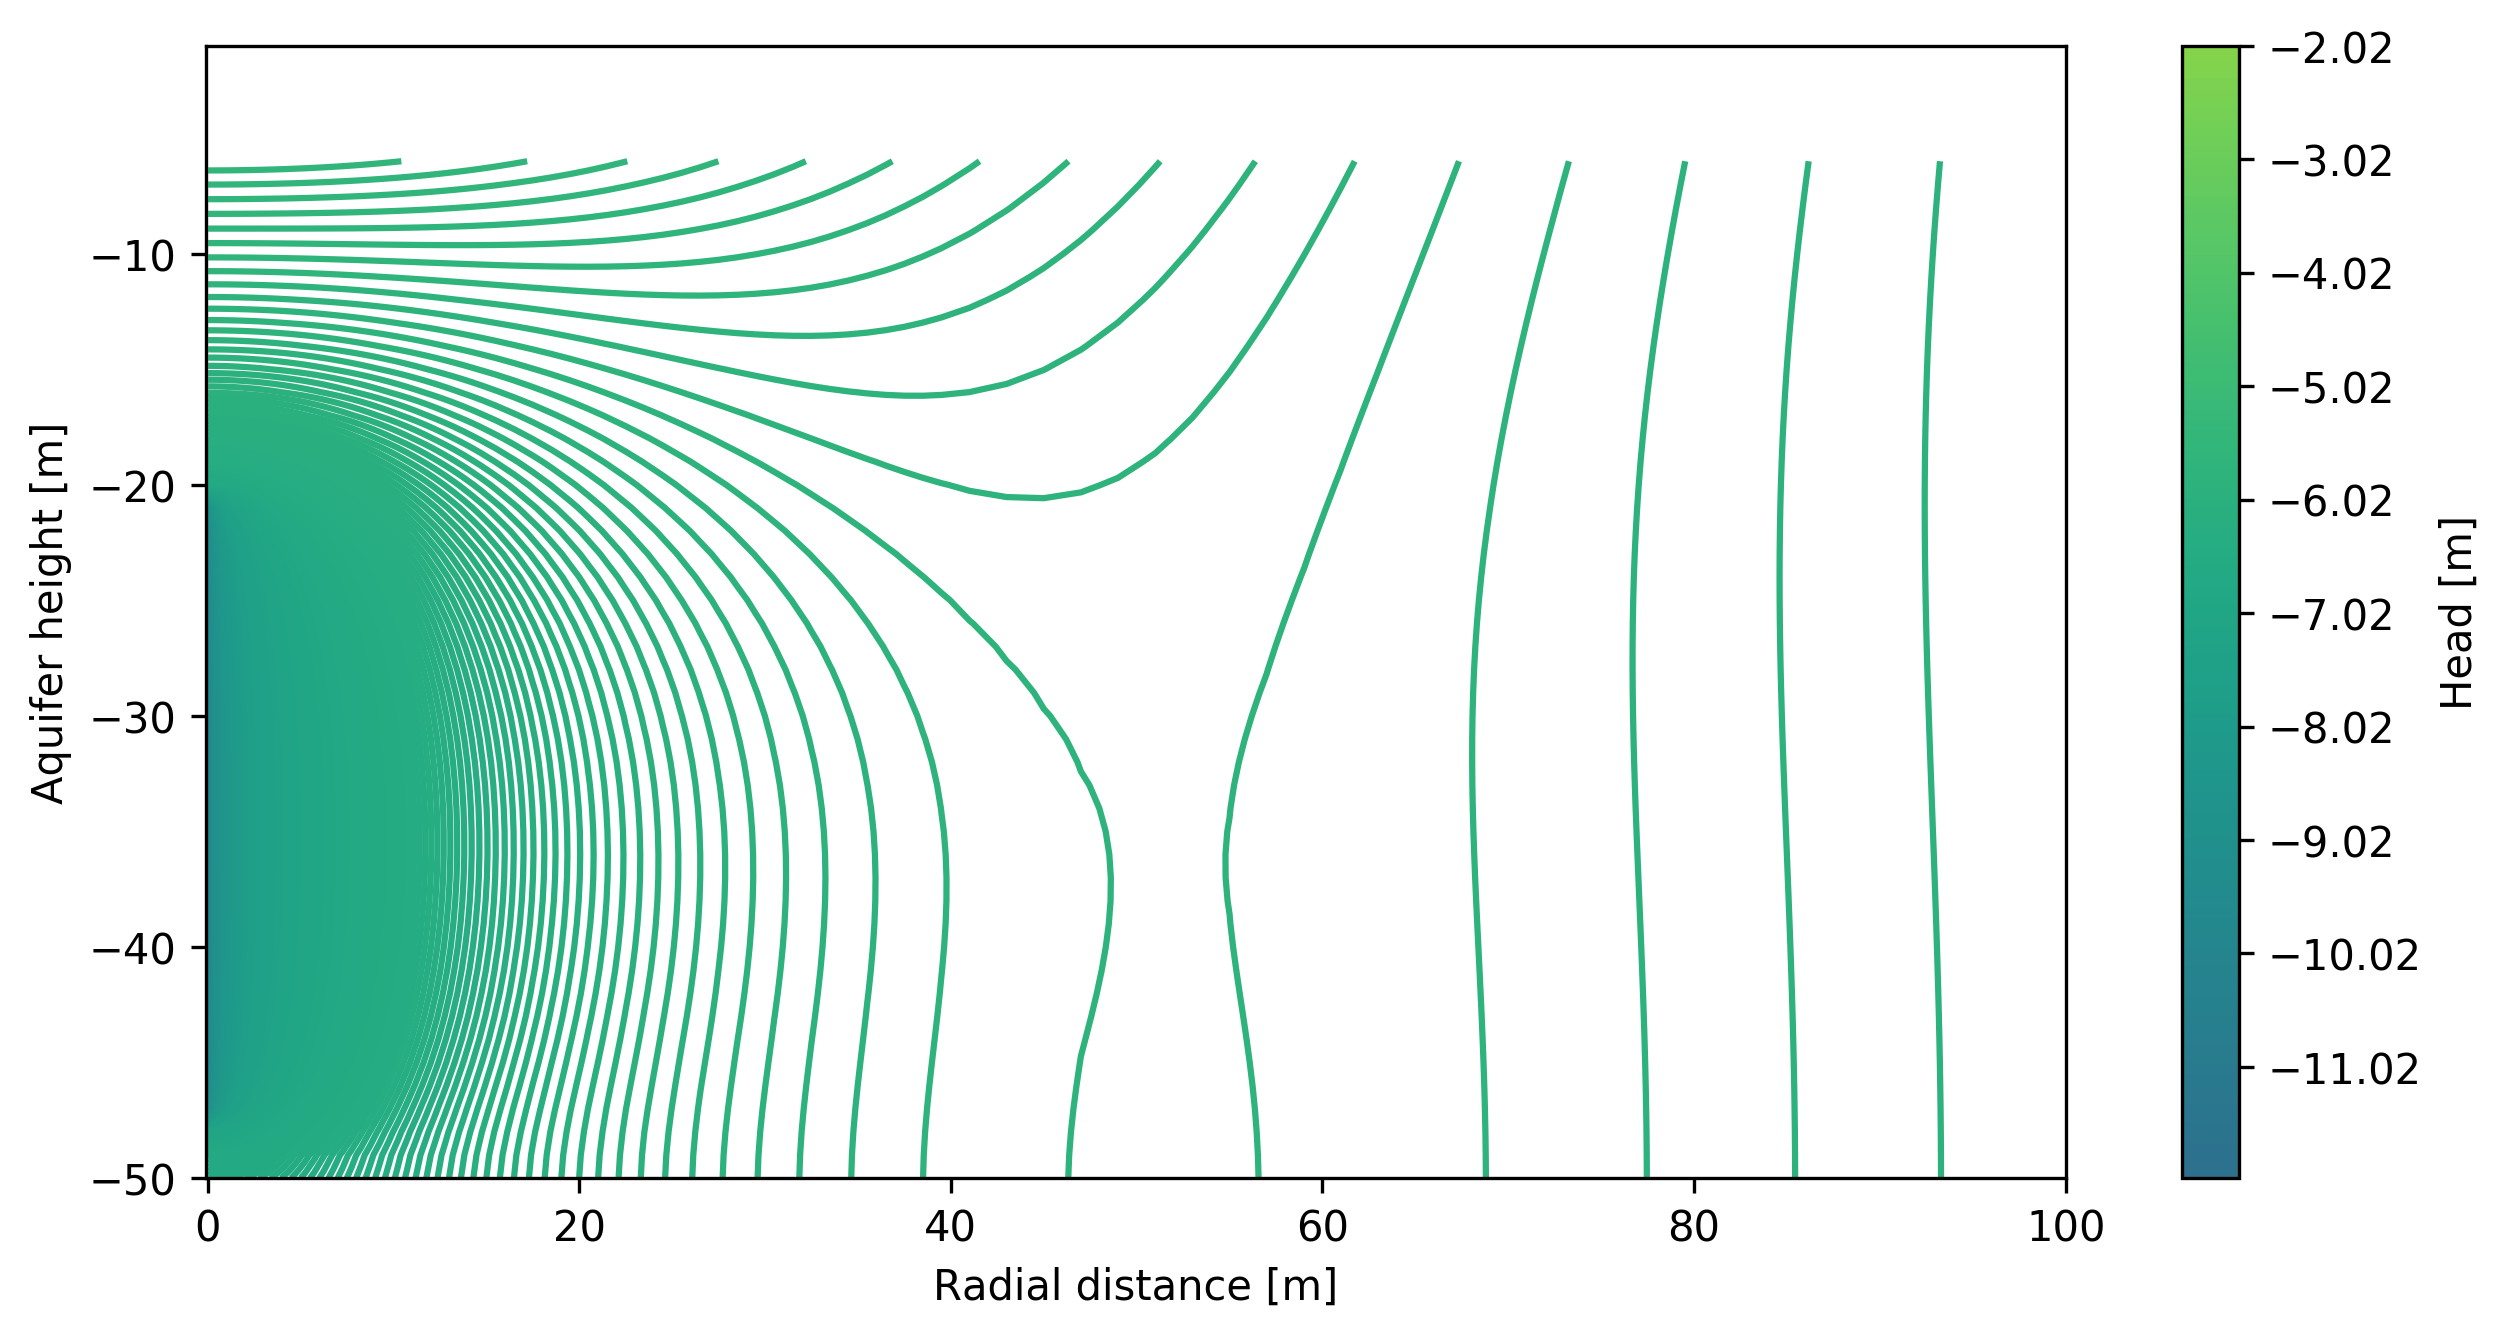
\includegraphics[width=\linewidth]{Sc3a1_cont_d123pump}
		\captionsetup{justification=centering}		
		\caption{\label{fig:Sc3a1_cont_d123pump}}
		\end{subfigure}\hfill
	\begin{subfigure}[b]{0.5\linewidth}
        \centering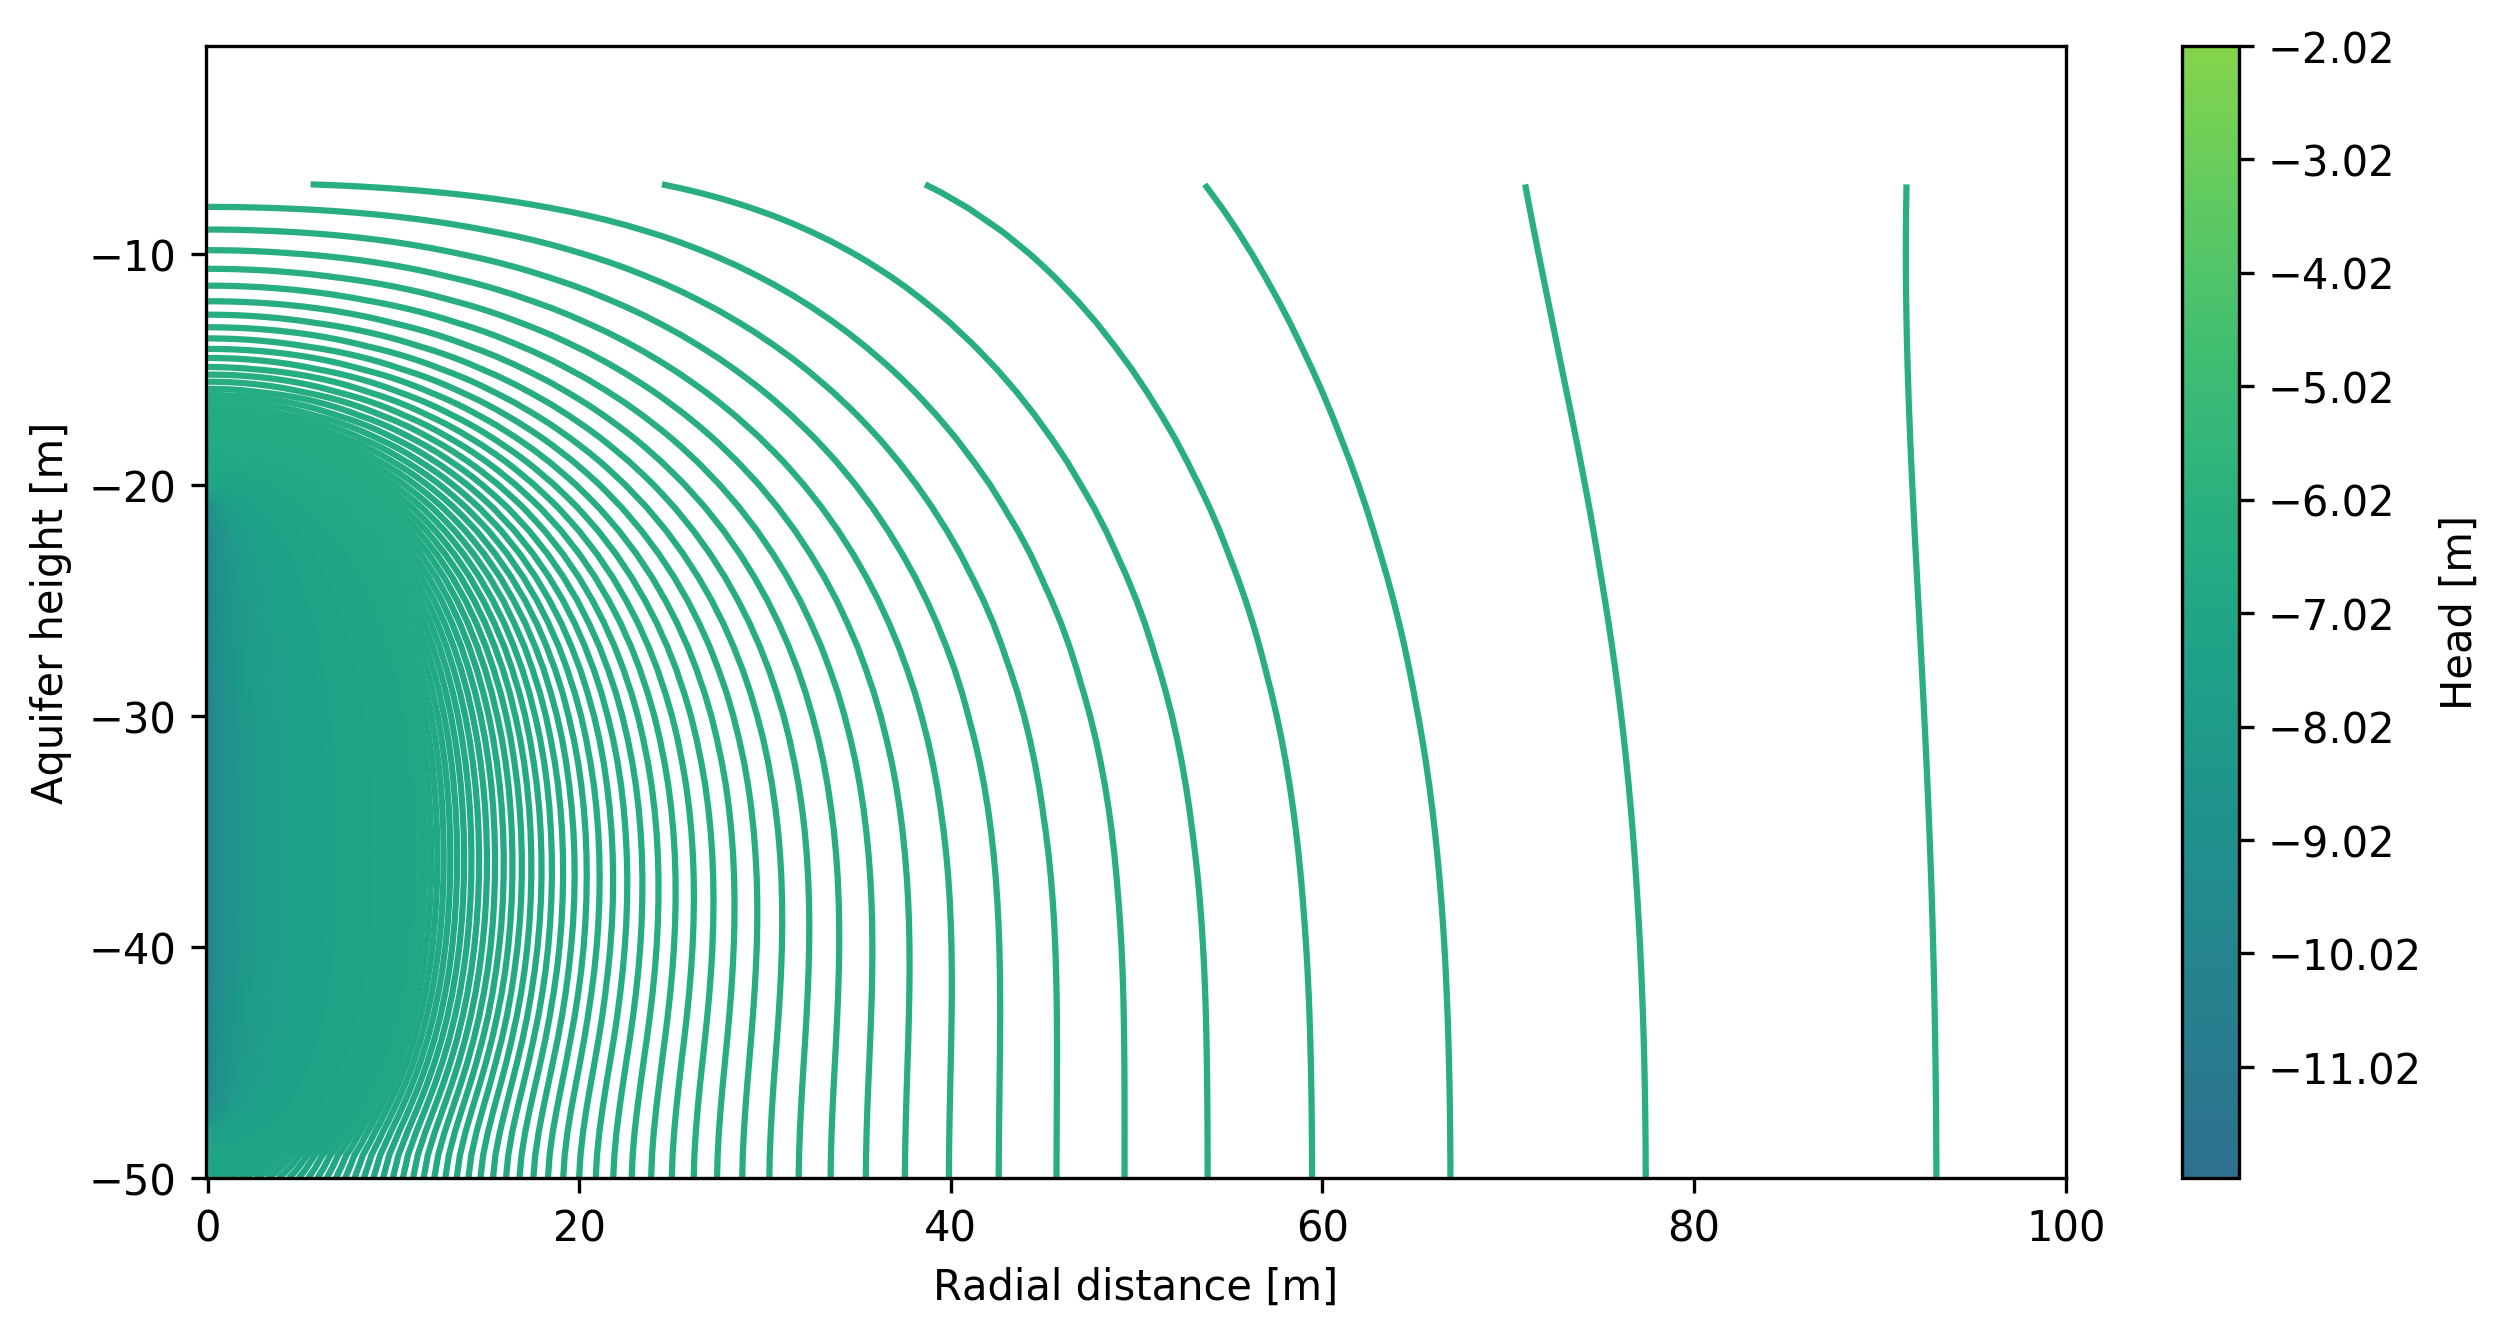
\includegraphics[width=\linewidth]{Sc3a1_cont_d364pump}
		\captionsetup{justification=centering}		
		\caption{\label{fig:Sc3a1_cont_d364pump}}
		\end{subfigure}
		\captionsetup{justification=centering}	
	\caption{Example scenario 3 - base model - Cross-sectional contour head after four hours of pumping on (\subref{fig:Sc3a1_cont_d123pump}) the first day (day 123) and (\subref{fig:Sc3a1_cont_d364pump}) the last day (day 365) of dry season} 
	\label{fig:Example_Sc3_base_cont_dry}
\end{figure} 

The impact of well discharge is visualized for scenario 3 in both, a cross sectional contour plot (Figure \ref{fig:Example_Sc3_base_cont_dry}) and a figure of groundwater heads in representative model layers over radial distance (Figure \ref{fig:Example_Sc3_base_head_dry}). After the first day of pumping the transition from wet (recharge) to dry season (discharge) is still of influence. Most definitely in the higher model layers (close to surface) the increased heads (due to wet season recharge) remain active for some time. Towards the end of dry season this impact is no longer present. Over the entire dry season the predefined bound in head (-20 m) is not reflected in the visualized heads. This can be justified by the presence of a well skin resistance. Bounded drawdown is only reached within the well. As a result, the consequences on nature (groundwater) are less distinct.   

\begin{figure}[h!]
	\centering
	\begin{subfigure}[b]{0.5\linewidth}
		\centering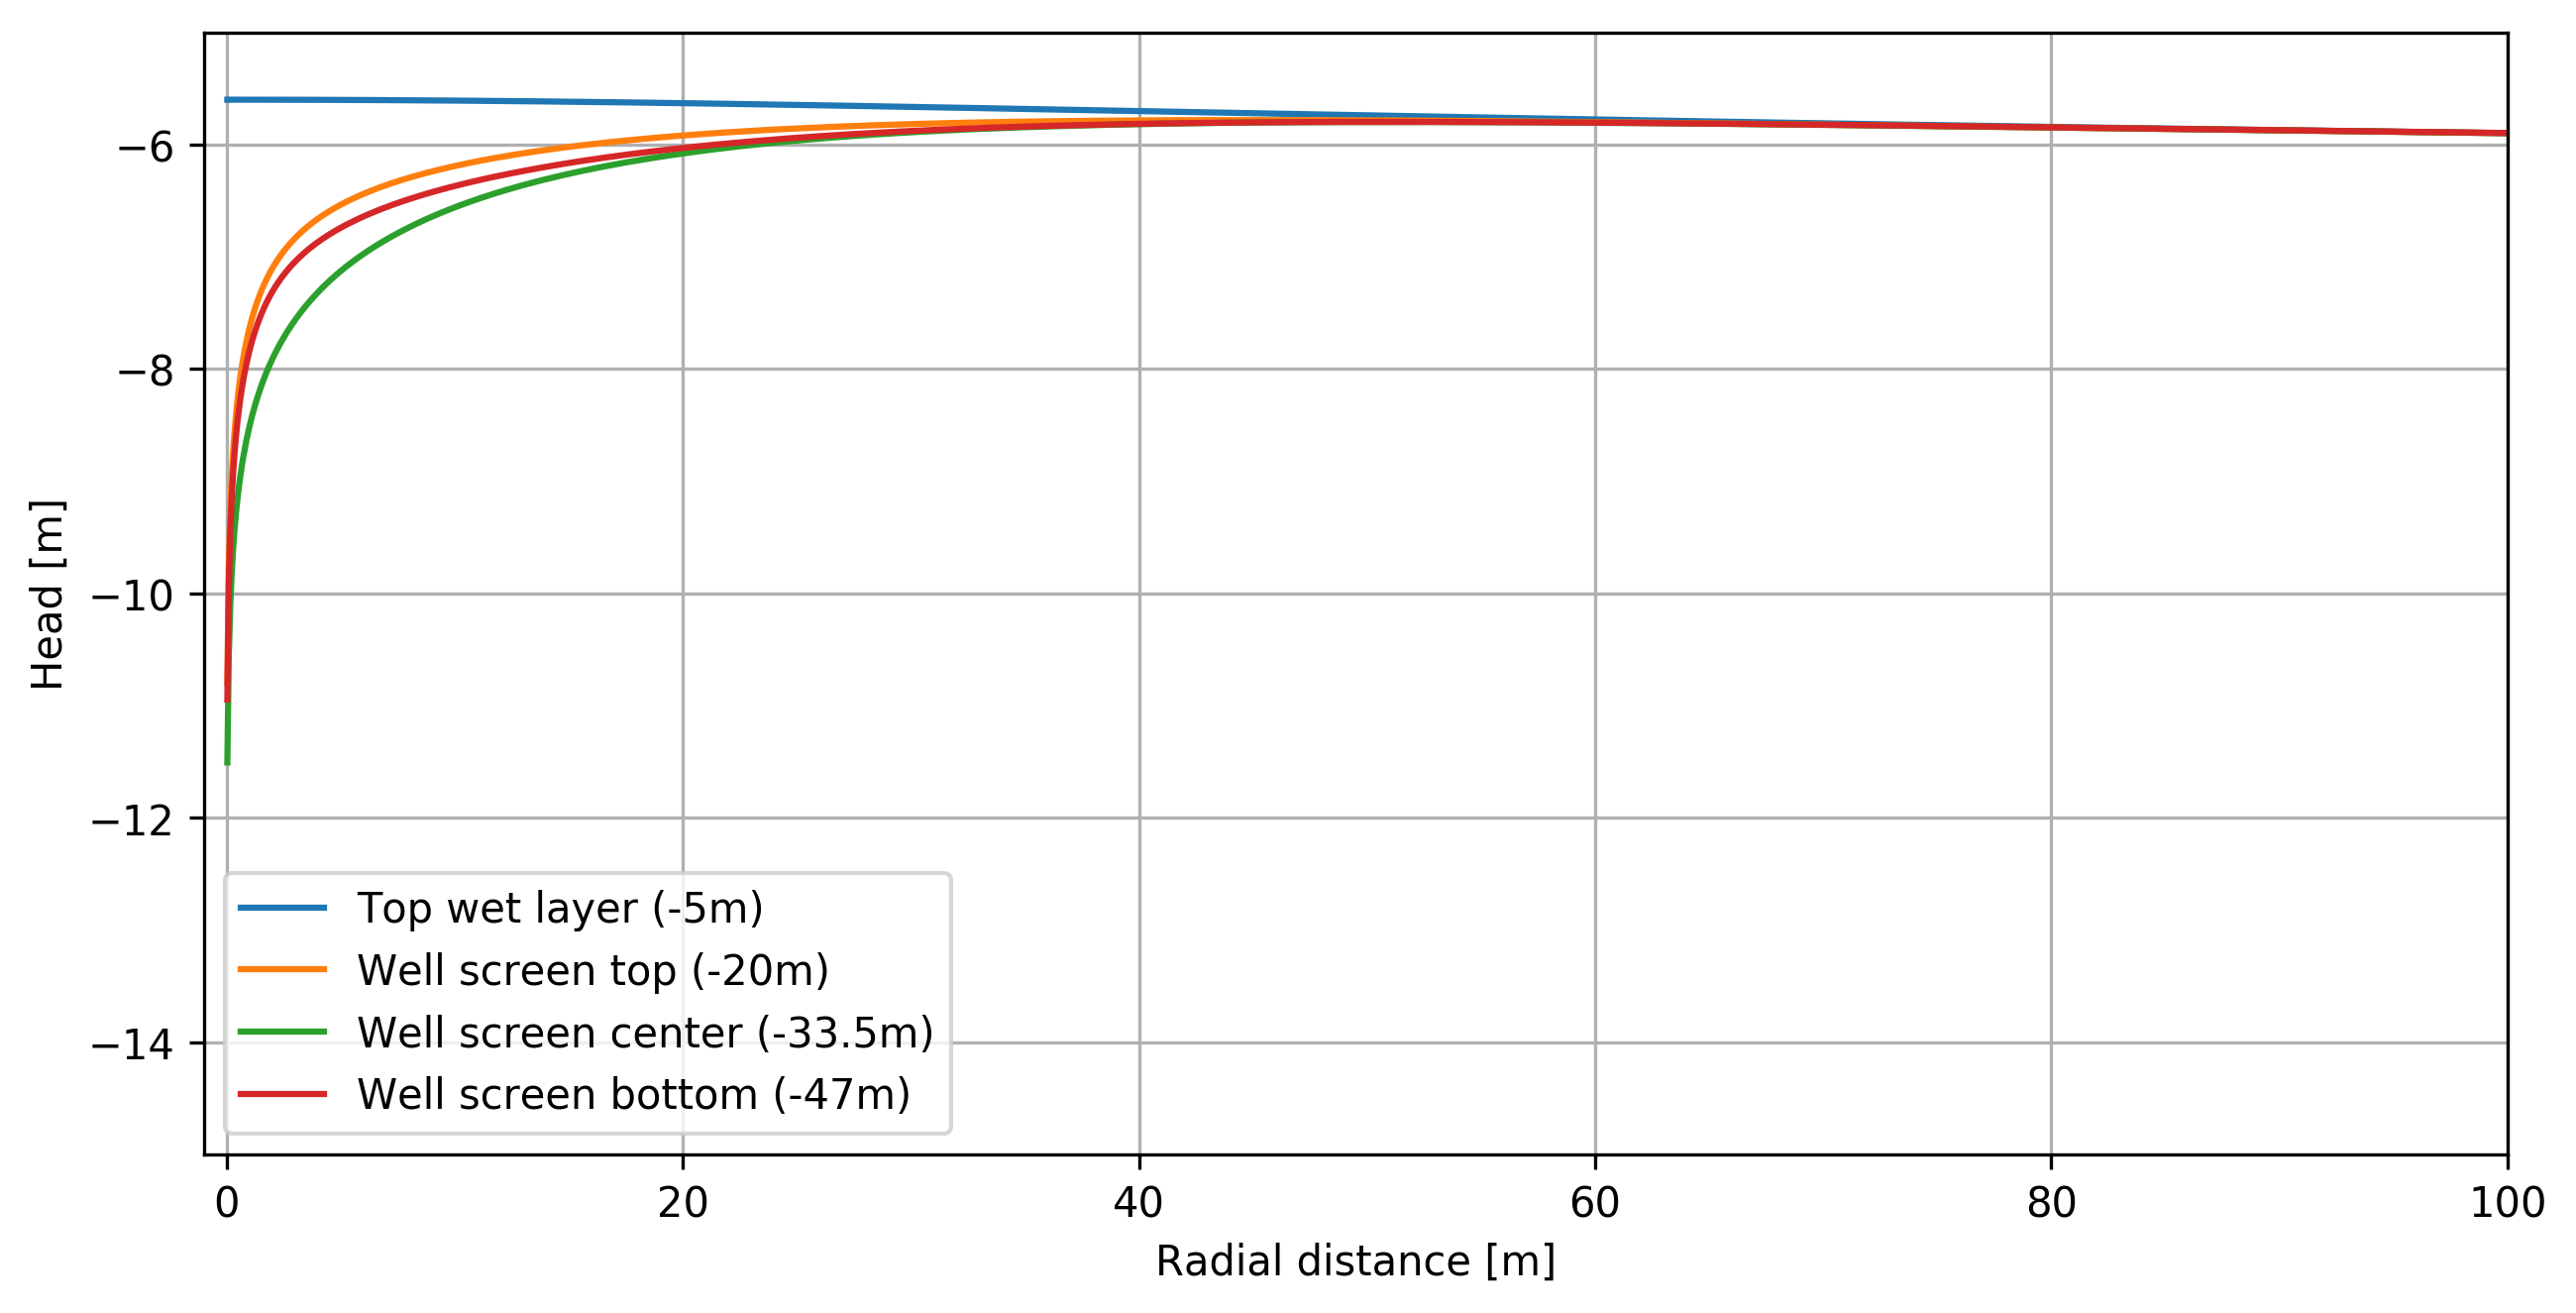
\includegraphics[width=\linewidth]{Sc3a1_head_d123pump}
		\captionsetup{justification=centering}		
		\caption{\label{fig:Sc3a1_head_d123pump}}
		\end{subfigure}\hfill
	\begin{subfigure}[b]{0.5\linewidth}
        \centering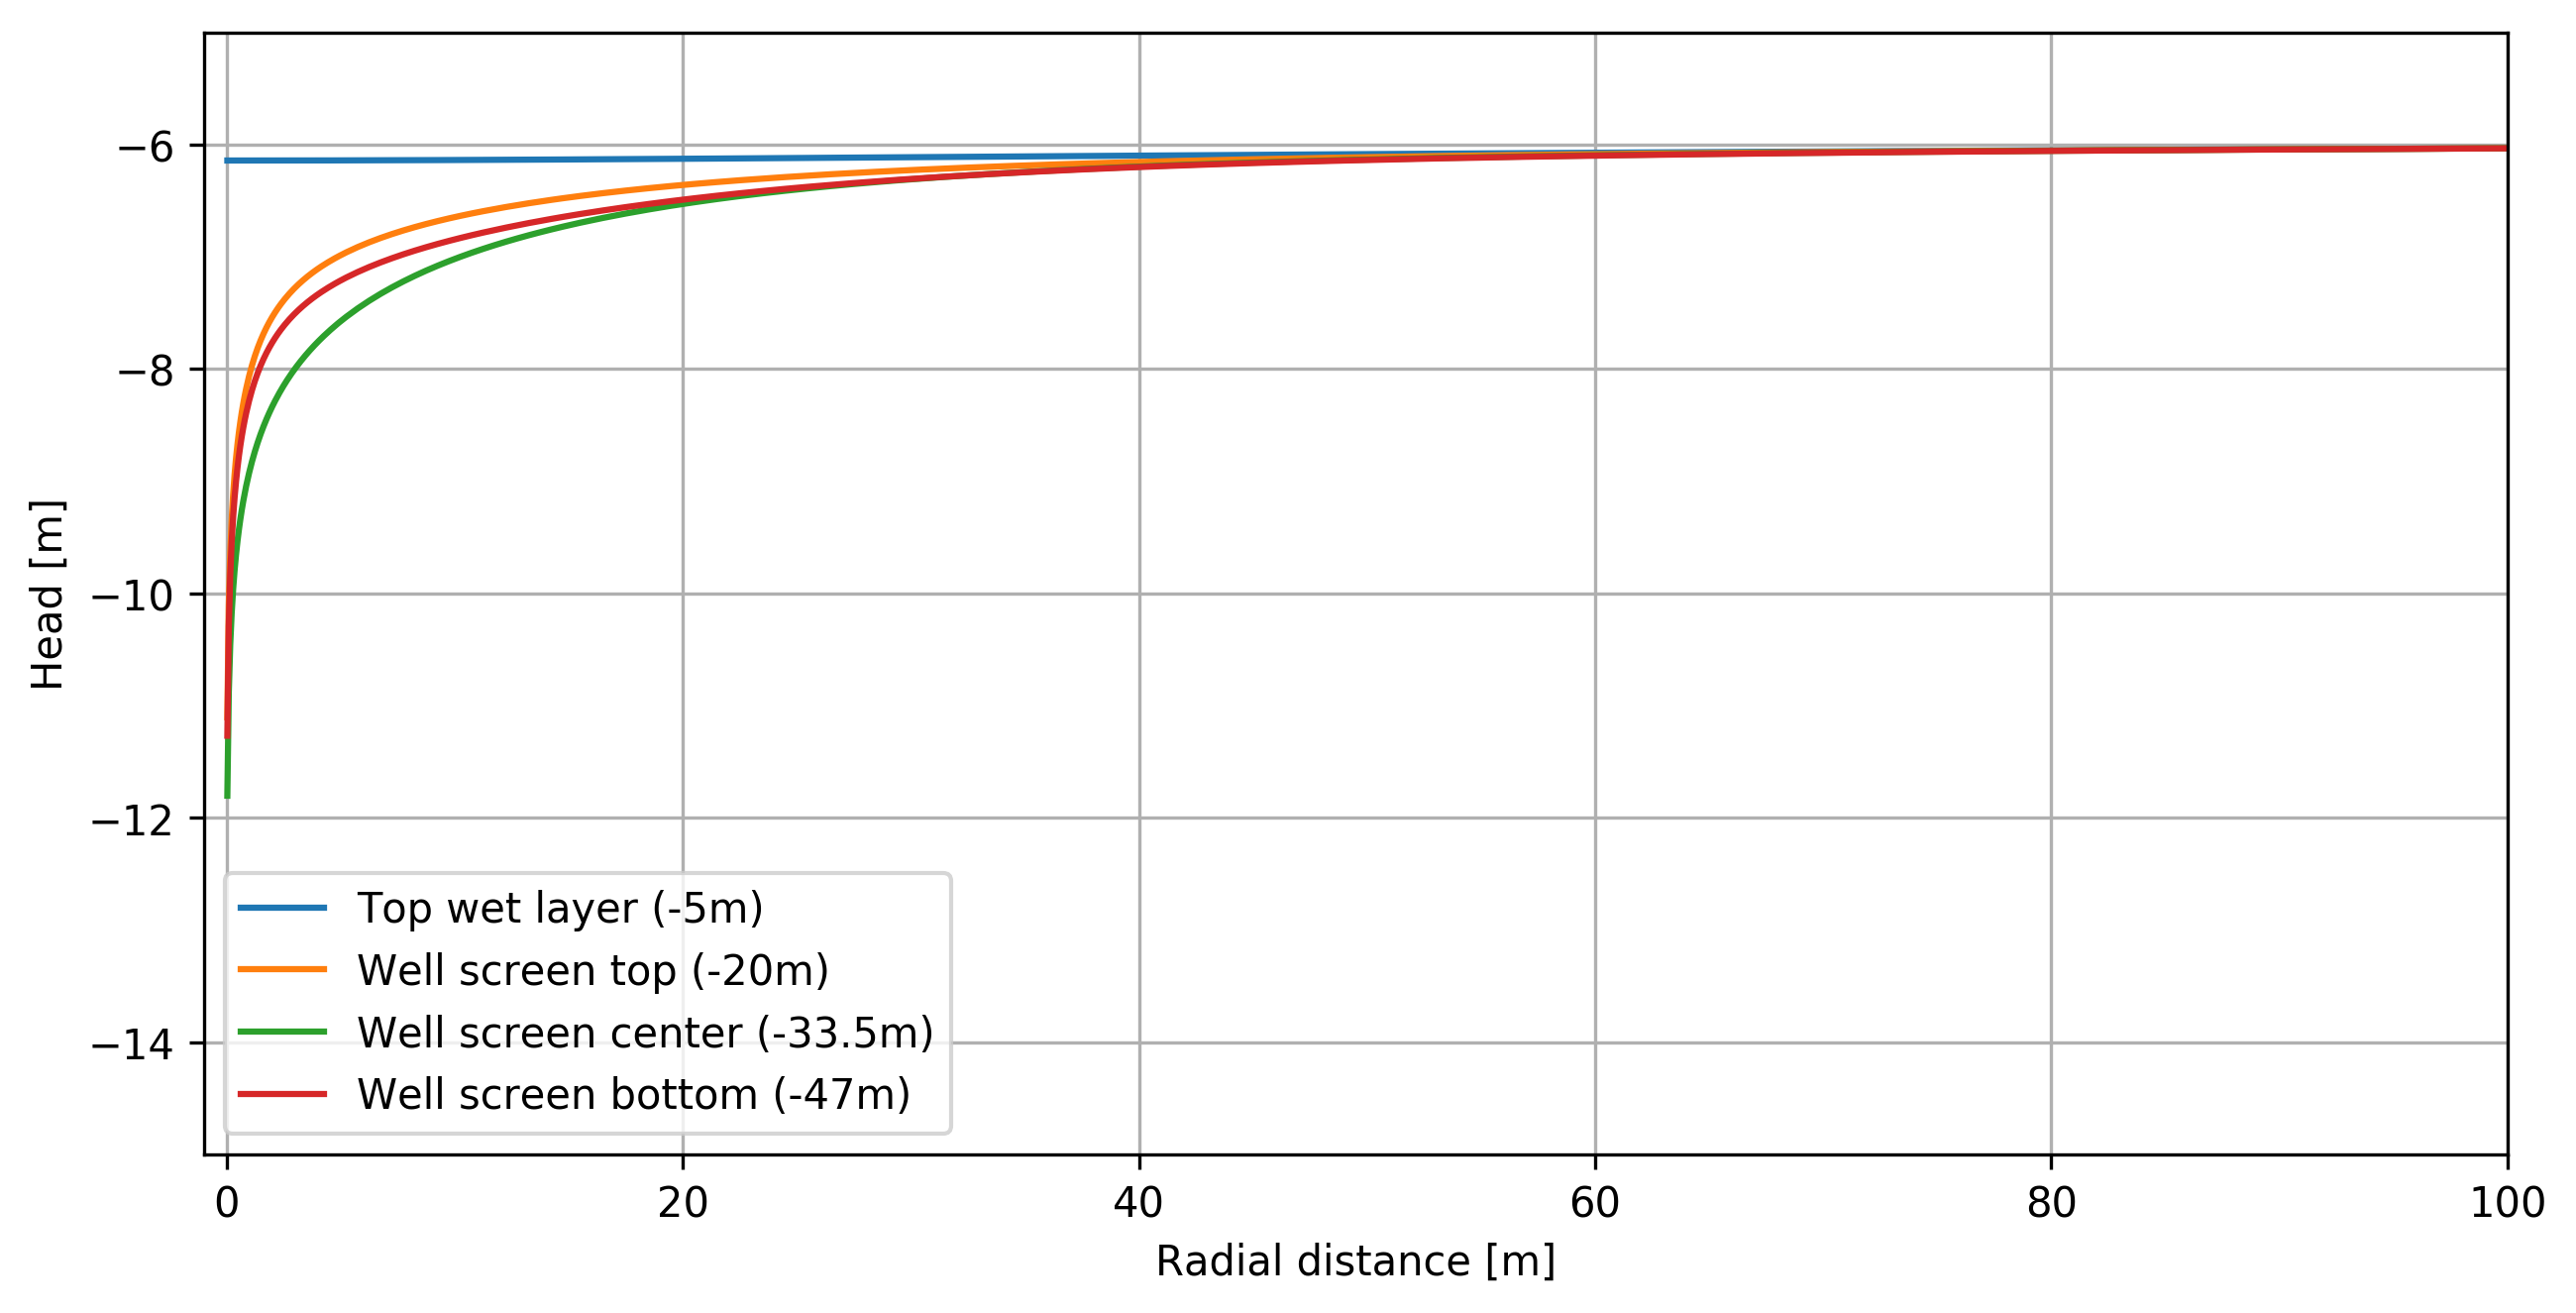
\includegraphics[width=\linewidth]{Sc3a1_head_d364pump}
		\captionsetup{justification=centering}		
		\caption{\label{fig:Sc3a1_head_d364pump}}
		\end{subfigure}
		\captionsetup{justification=centering}	
	\caption{Example scenario 3 - base model - Head in representative layers after four hours of pumping on (\subref{fig:Sc3a1_head_d123pump}) the first day (day 123) and (\subref{fig:Sc3a1_head_d364pump}) the last day (day 365) of dry season} 
	\label{fig:Example_Sc3_base_head_dry}
\end{figure} 

Unlike the outcomes in recharge (wet season) the soil scenarios show distinctive results in total volumes discharged. It can be suggested the variation in storativity is more pronounced for discharge (after a certain time of recharge). However the differences in total volumes withdrawn are still in the same order of size for the scenarios 1 and 2 as well as the scenarios 4 and 5. 

\begin{table}[h!]
\small
\centering
\caption{Base model scenarios - Dry season discharge (m3)}
\label{tab:Base_discharge}
\begin{tabular}{l|r|r|r|r|r}
\hline 
\textbf{}               & \textbf{Sc 1} & \textbf{Sc 2} & \textbf{Sc 3} & \textbf{Sc 4}  & \textbf{Sc 5} \\ \hline \hline
Volume out (m$^3$)       & 199.25        & 218.13        & 3310.17       & 6161.15 	      & 6232.08          \\ \hline    
\end{tabular}
\end{table}

\textbf{Year-round recovery ratio $R_\%$} \\
Recovery ratios are for all base models scenarios in the same order of size (Table \ref{tab:Base_RR}. Mutual differences can potentially be attributed to the varying behaviour of storativity (in combination with different transmissivity values). The ratios are however also affected by the (scenario dependent) well skin resistances. As a consequence, no distinctive conclusions on scenario comparison can be drawn. \\ 

\begin{table}[h!]
\small
\centering
\caption{Base model scenarios - Recovery ratio $R_\%$}
\label{tab:Base_RR}
\begin{tabular}{l|r|r|r|r|r}
\hline 
\textbf{}               & \textbf{Sc 1} & \textbf{Sc 2} & \textbf{Sc 3} & \textbf{Sc 4}  & \textbf{Sc 5} \\ \hline \hline
$R_\%$ (-)              &  0.649        & 0.705         & 0.616         & 0.588 	     & 0.594 	          \\ \hline    
\end{tabular}
\end{table}

In all base scenarios the recovery ratio stays well below 1. In eight months of daily (4 hours) pump operation it is not possible to fully recover the volumes infiltrated due to four months of constant inundation (2 meter) on top of a well. Under the defined conditions of system composition and use, the found recovery ratios suggest a sustainable system impact on nature. 

%\clearpage
\section{Impact of ASR-system upscaling}
\label{section:ASR_upscaling}
This section elaborates on the impact of ASR-system upscaling. One-by-one the different types of upscaling (pumping time, dimension and cleaning) are taken into account. Performances are tested and compared to the base model by the known parameters: total recharge, total discharge and the recovery ratio ($R_{\%}$).  

\tikzstyle{mybox} = [draw=black, fill=white, very thick,
    rectangle, rounded corners, inner sep=20pt, inner ysep=20pt]
\tikzstyle{title} =[fill=black, text=white]

\subsection{Upscaling daily pumping time}
\label{Subsec:Up_time}
ASR-system upscaling by an extent in (dry season) daily pump operation is easily applicable. Except from additional fuel and possibly temporal storage requirements (poly tanks), no further modifications are required. Base model pump operation is set to be four hours daily (243 days, dry season). This study is pointed at a maximum time-scope of 12 hours daily. A four-steps distinction is made in upscaling (6h, 8h, 10h and 12h), as mentioned in Figure \ref{fig:Schematic_up_time}. 

\begin{figure}[H]
\centering
\begin{tikzpicture}
\node [mybox] (box){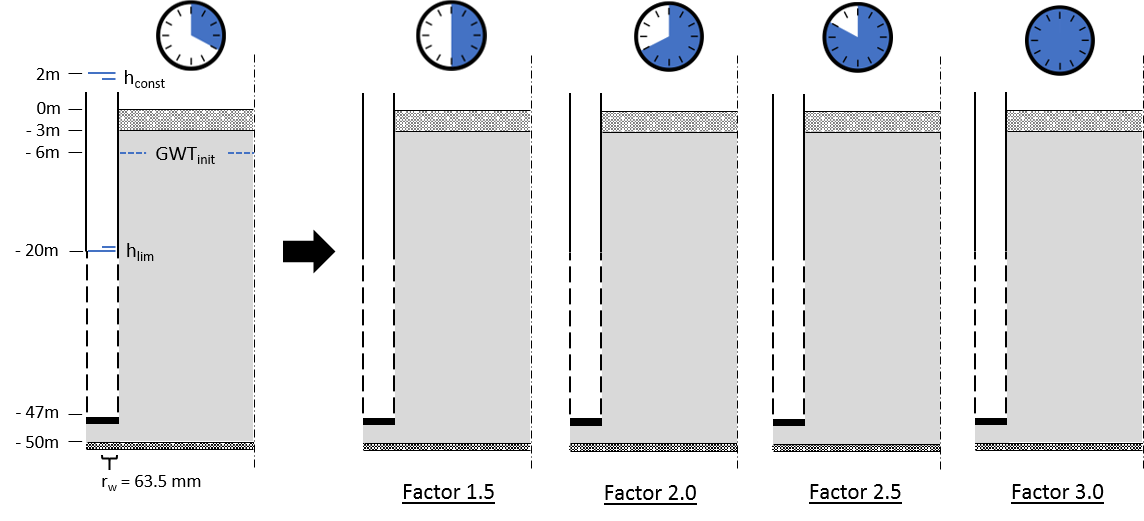
\includegraphics[width=0.9\linewidth]{Schematic_up_time}};  
\node[title, right=10pt] at (box.north west) {Schematic upscaling daily pumping time};
\end{tikzpicture}
\captionsetup{justification=centering}
\caption{Schematic upscaling daily pumping time}
\label{fig:Schematic_up_time}
\end{figure}

Deviations in wet season recharge are not applicable to upscaling by pump duration. Pump operation is in effect during dry season only. As visible in Figure \ref{fig:Results_up_time}, discharged volumes are most definitely affected by daily pump duration. An approximately linear relation is encountered in all scenarios. The relation can be justified by the daily discharge performance as depicted for the base model in Figure \ref{fig:Example_Sc1_base_discharge}. After four hours of pumping a more or less equilibrium discharge rate is encountered. Expansion by adding active hours of pumping daily will not make any significant change in discharge rates. Moreover, the discharge pattern is repeated daily. Mutual differences between the days of pump operation are absent. \\

\begin{figure}[h!]
 \centering
 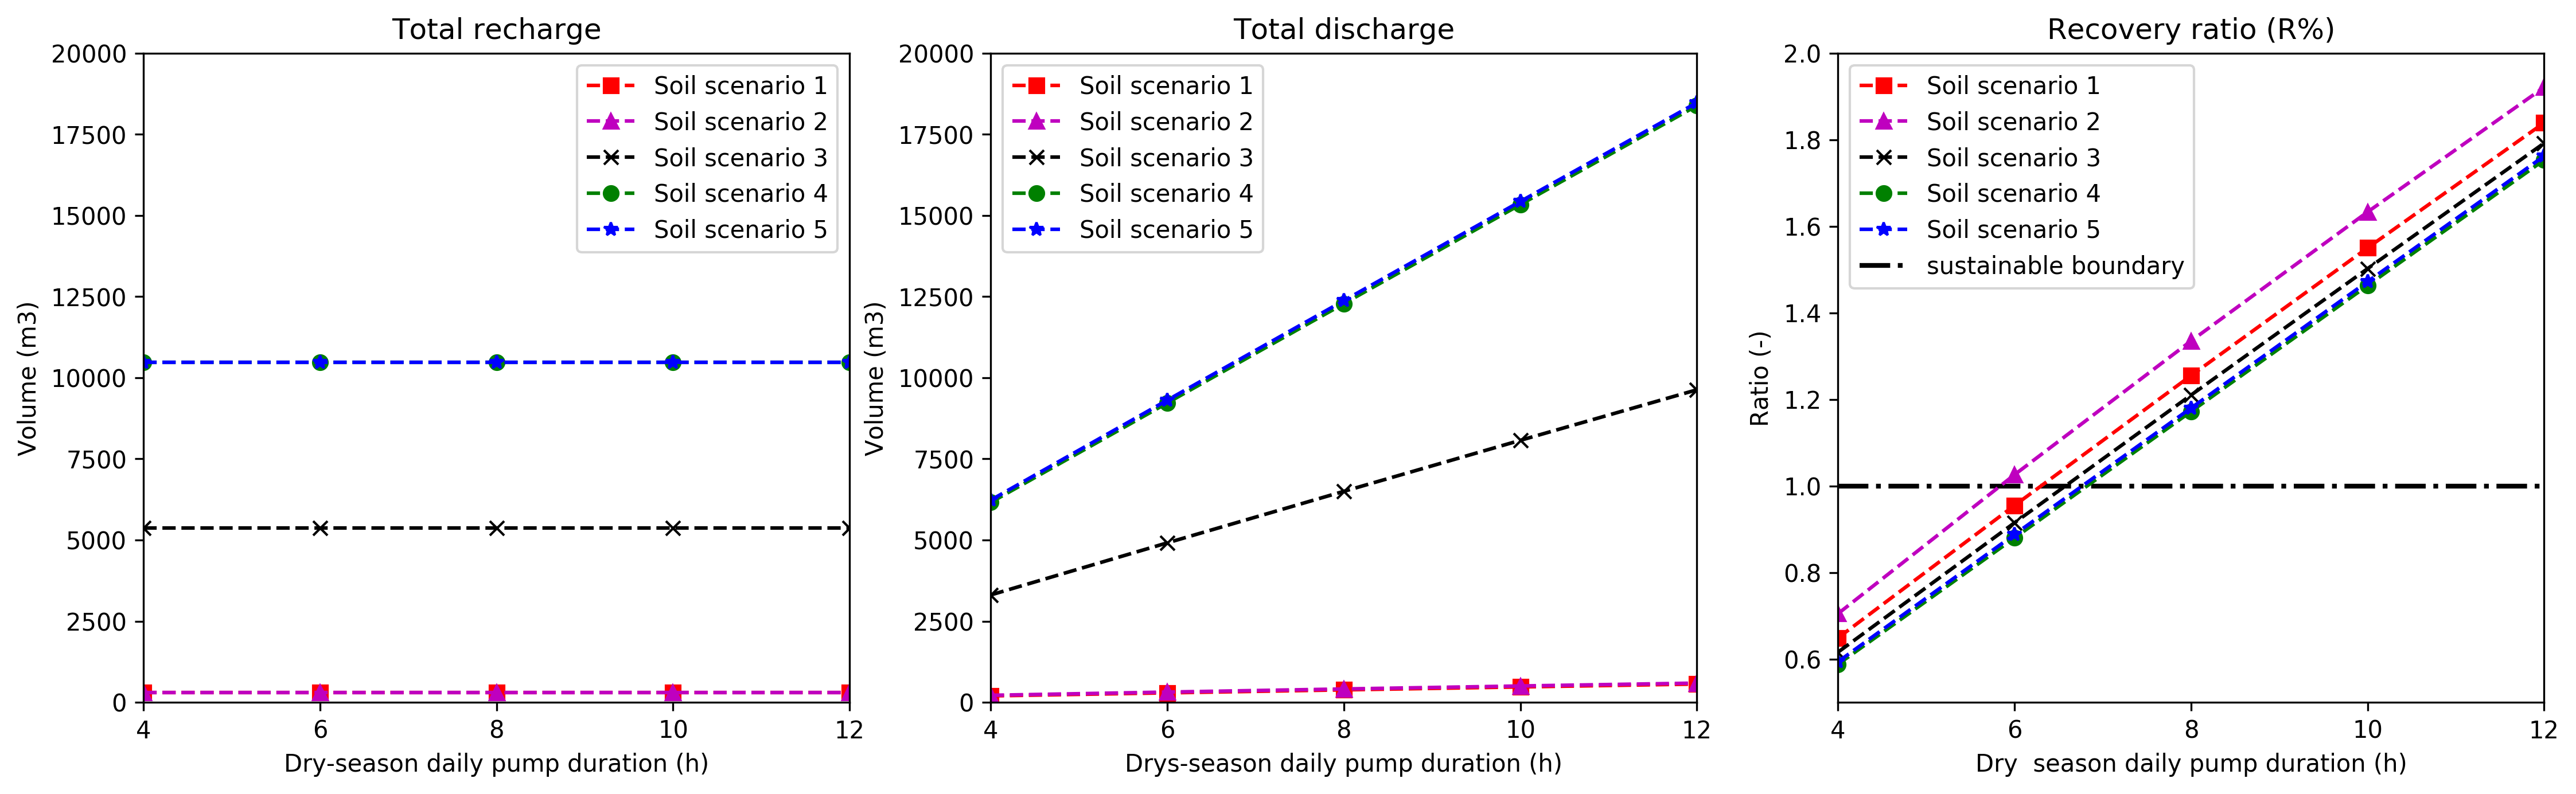
\includegraphics[width=1.0\linewidth]{Results_up_time}
 \captionsetup{justification=centering} 
 \caption{Results of yearly total volumes (in, out, ratio) by upscaling daily pumping time}
 \label{fig:Results_up_time}
\end{figure}

Discharge volumes obtained by upscaling daily pump duration for the total eight months of dry season exceed the four months (gravity based) recharge volumes. under the applied conditions of maximum upscaling (12u daily; total pumping time equals duration wet season) recovery ratio close to two are reached. By scaled-up pump duration the potential negative effects on nature (unsustainable system use) should be considered.

\subsection{Upscaling borehole cross-sectional dimension}
\label{Subsec:Up_diam}
ASR-system upscaling by an increase in borehole dimension is a rigorous approach. An adjustment that can not be applied on existing systems. If the appropriate equipment is present (e.g. drilling machinery), new construction of enlarged ASR-systems can be applied. To take implementation in consideration it is of extra interest to gain knowledge on potential effects. Simulation is executed by stepwise (4 steps) doubling the original borehole radius (Figure \ref{fig:Schematic_up_diam}). 

\begin{figure}[h!]
\centering
\begin{tikzpicture}
\node [mybox] (box){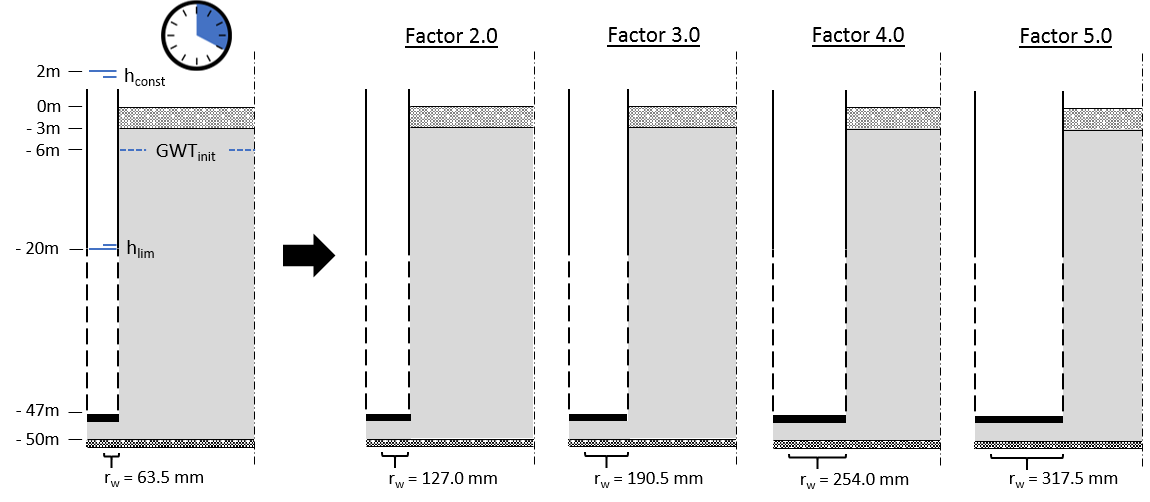
\includegraphics[width=0.9\linewidth]{Schematic_up_diam}};  
\node[title, right=10pt] at (box.north west) {Schematic upscaling borehole cross-sectional dimension};
\end{tikzpicture}
\captionsetup{justification=centering}
\caption{Schematic upscaling borehole cross-sectional dimension}
\label{fig:Schematic_up_diam}
\end{figure}

Magnification of the borehole diameter is beneficial for both groundwater recharge and discharge. Results show a non-linear relation between total season in- and outflow. Well-size upscaling has an increasingly less positive effect on the total volumes obtained. A further magnification has it limits.  

\begin{figure}[h!]
 \centering
 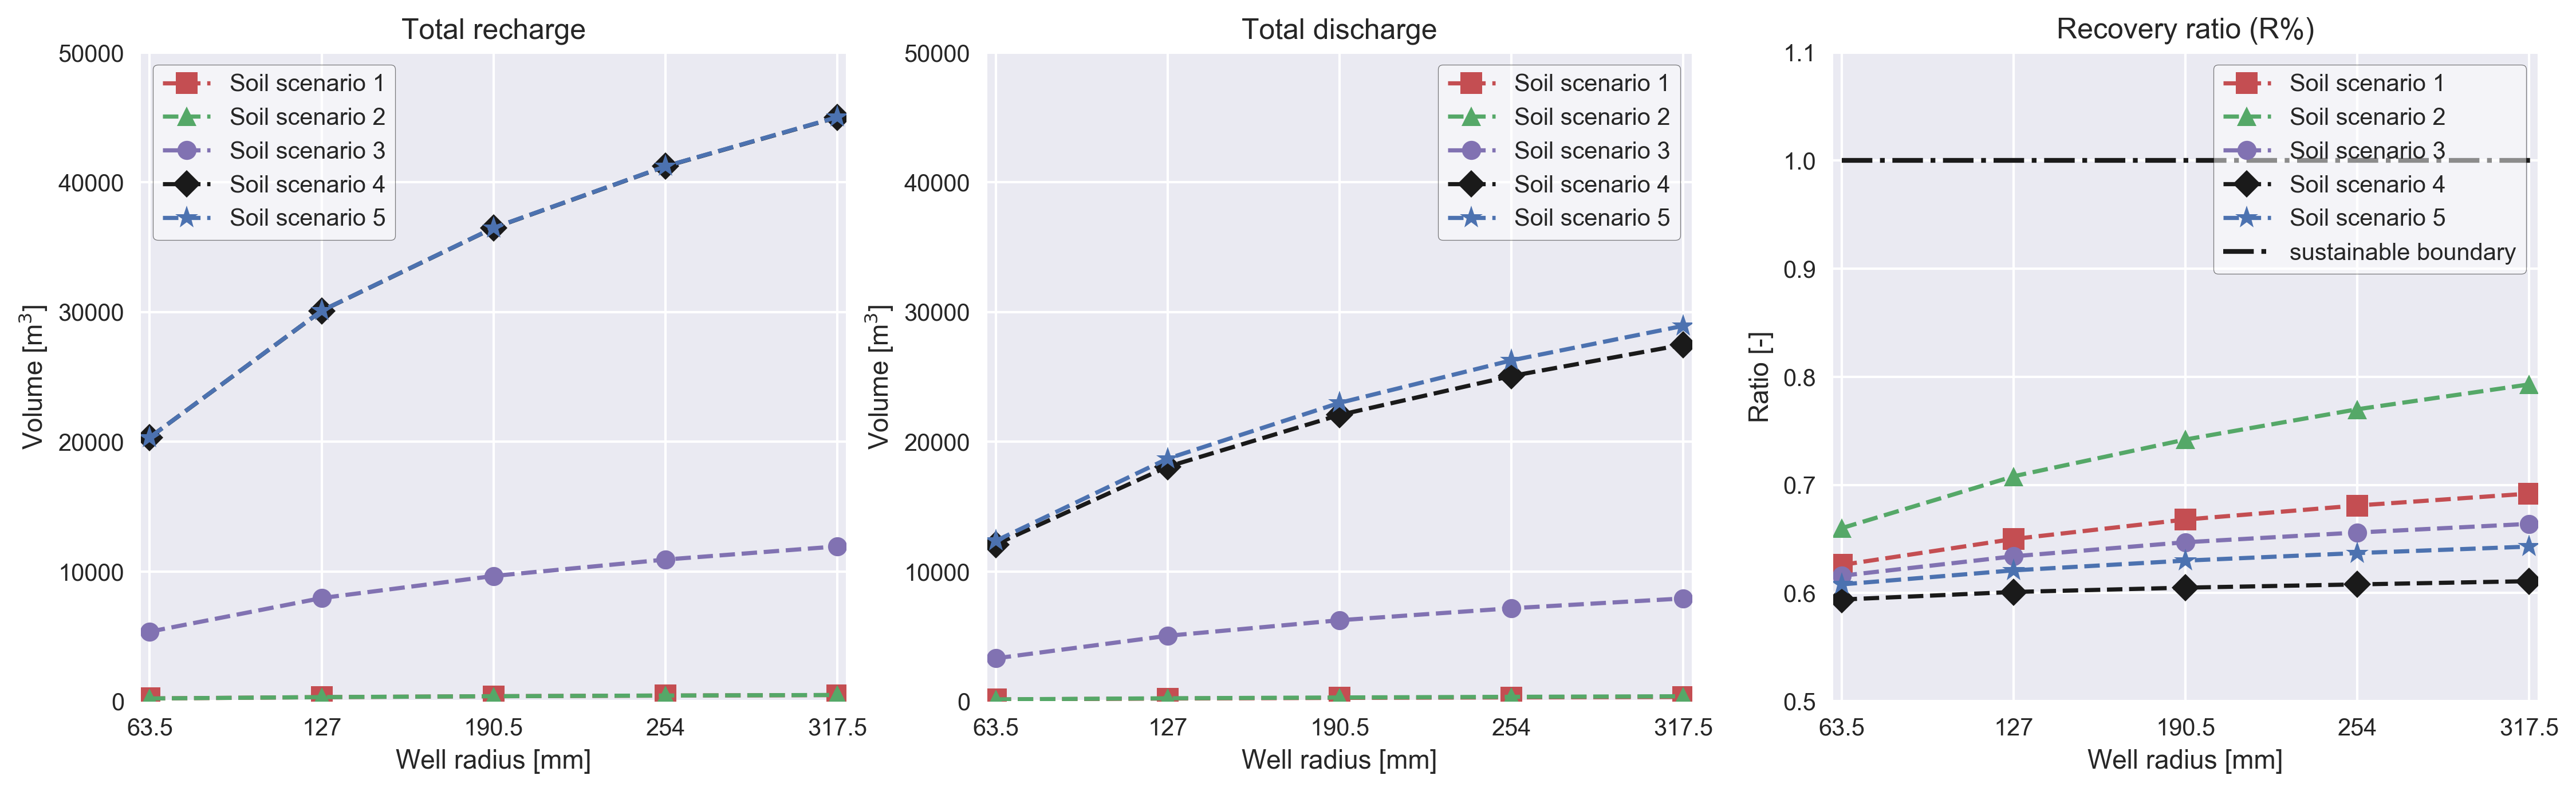
\includegraphics[width=1.0\linewidth]{Results_up_diam}
 \captionsetup{justification=centering} 
 \caption{Results of yearly total volumes (in, out, ratio) by upscaling well diameter}
 \label{fig:Results_up_diam}
\end{figure}

Unforeseen performances are obtained in the recovery ratios of scaled-up simulation in scenarios 1 and 2. After solid ratio increase, further system upscaling suddenly causes a decline in recovery performance. Closer inspection exposed the cause. Recharge volumes continue to follow an upward trend, while total discharge volumes stay at the same level. The predefined desired discharge ($Q_thiem$) are reached in these scaled-up scenarios. Impact becomes transparent by the comparison of discharge performances of the (soil) scenario 1 base model versus the model simulation with an (5 times) increased well radius (Figure \ref{fig:Example_Sc1_base_discharge} \& \ref{fig:Example_Sc1_5x_diam_discharge}). In these scenarios further well magnification results in a "release" of the head bound. Demands are met, while GWT is still in range. 

\begin{figure}[H]
	\centering
	\begin{subfigure}[b]{0.5\linewidth}
		\centering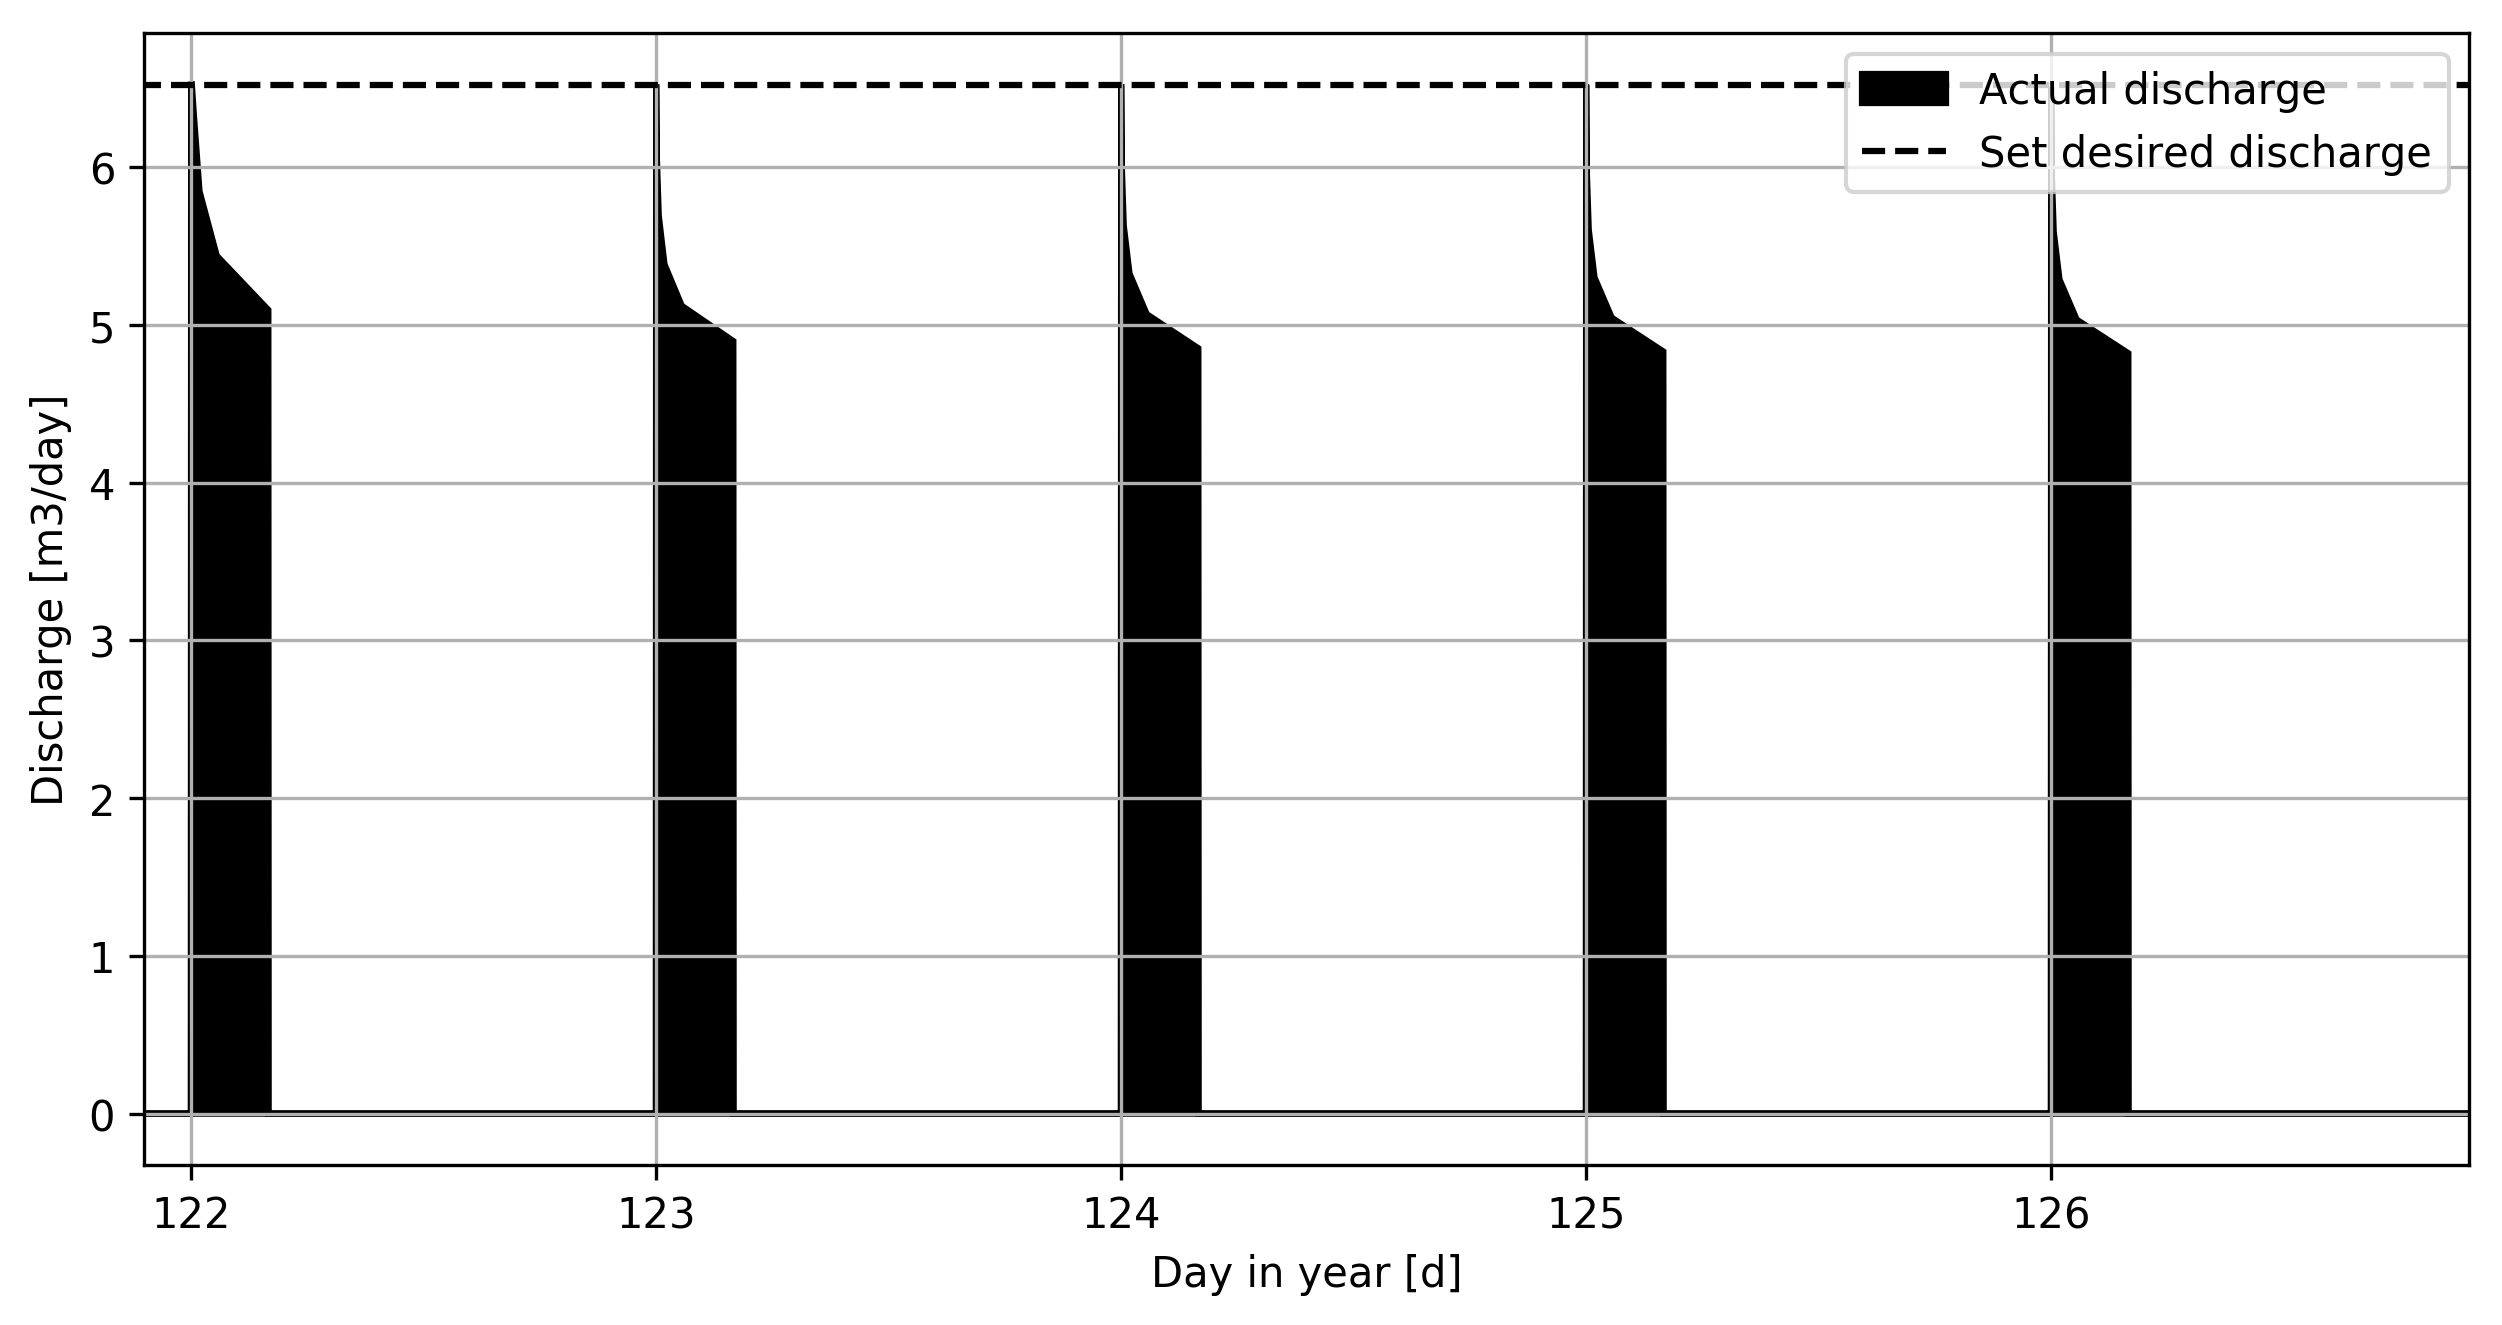
\includegraphics[width=\linewidth]{Sc1a1_Q122_126}
		\captionsetup{justification=centering}		
		\caption{\label{fig:Sc1a1_Q122_126}}
		\end{subfigure}\hfill
	\begin{subfigure}[b]{0.5\linewidth}
        \centering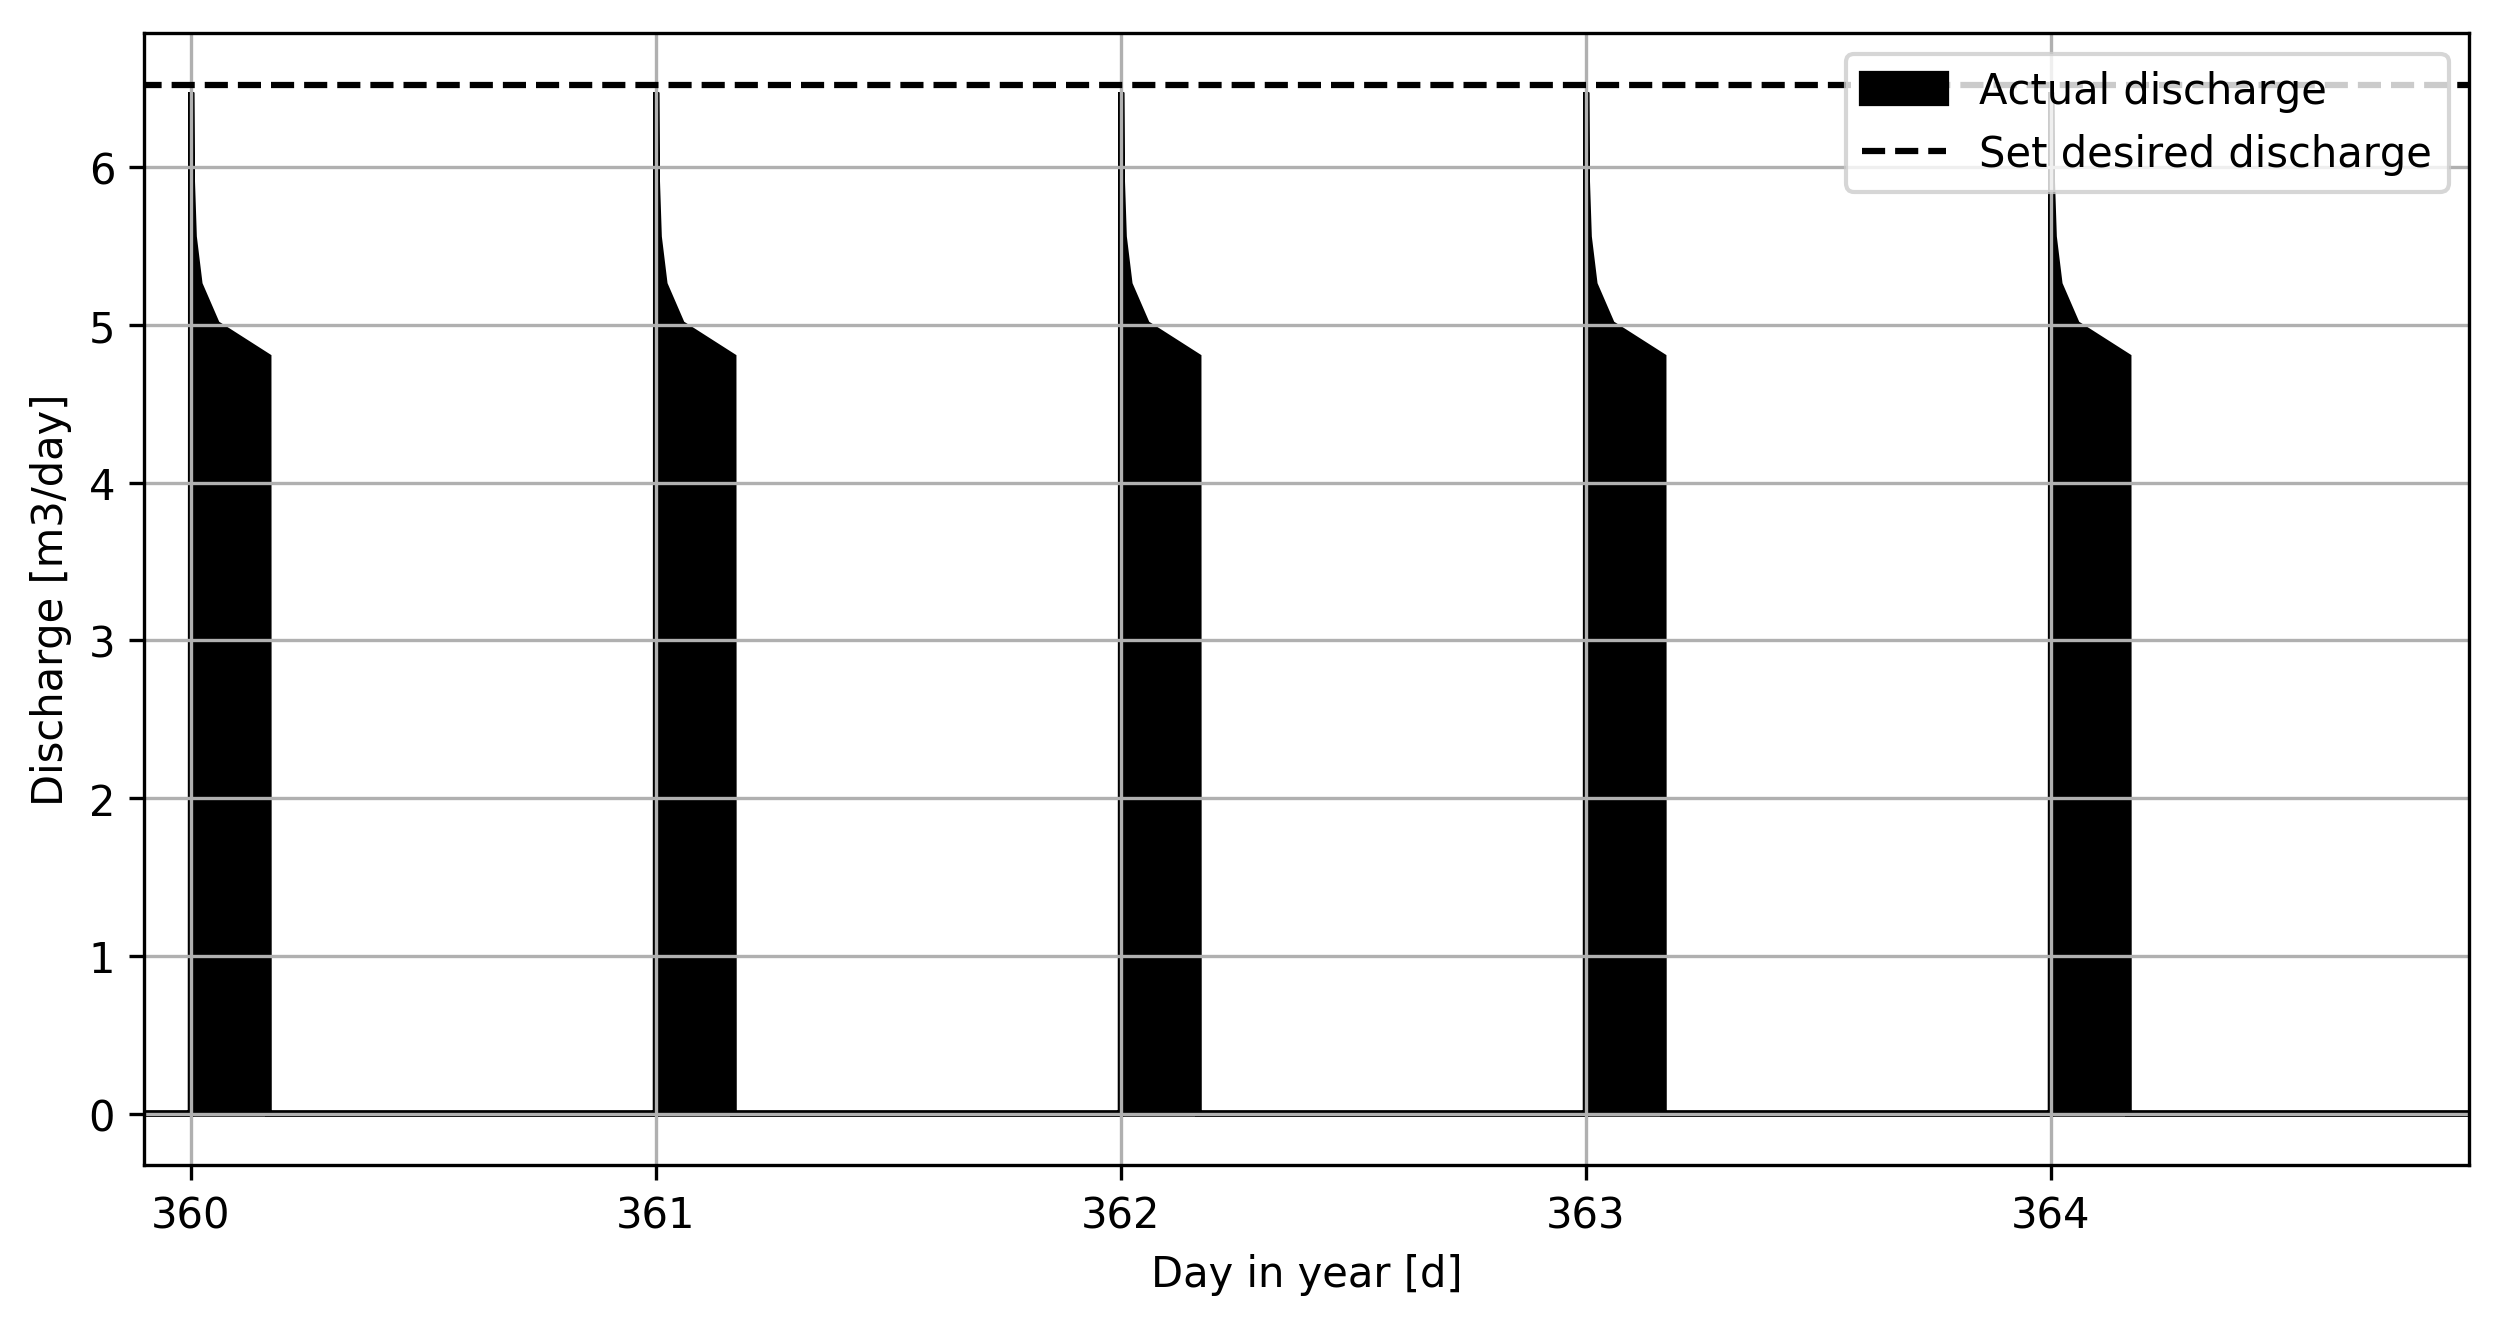
\includegraphics[width=\linewidth]{Sc1a1_Q360_364}
		\captionsetup{justification=centering}		
		\caption{\label{fig:Sc1a1_Q360_364}}
		\end{subfigure}
		\captionsetup{justification=centering}	
	\caption{Example scenario 1 - base model - Discharge performance for (\subref{fig:Sc1a1_Q122_126}) the first five days and (\subref{fig:Sc1a1_Q360_364}) the last five days of dry season} 
	\label{fig:Example_Sc1_base_discharge}
\end{figure} 

\begin{figure}[H]
	\centering
	\begin{subfigure}[b]{0.5\linewidth}
		\centering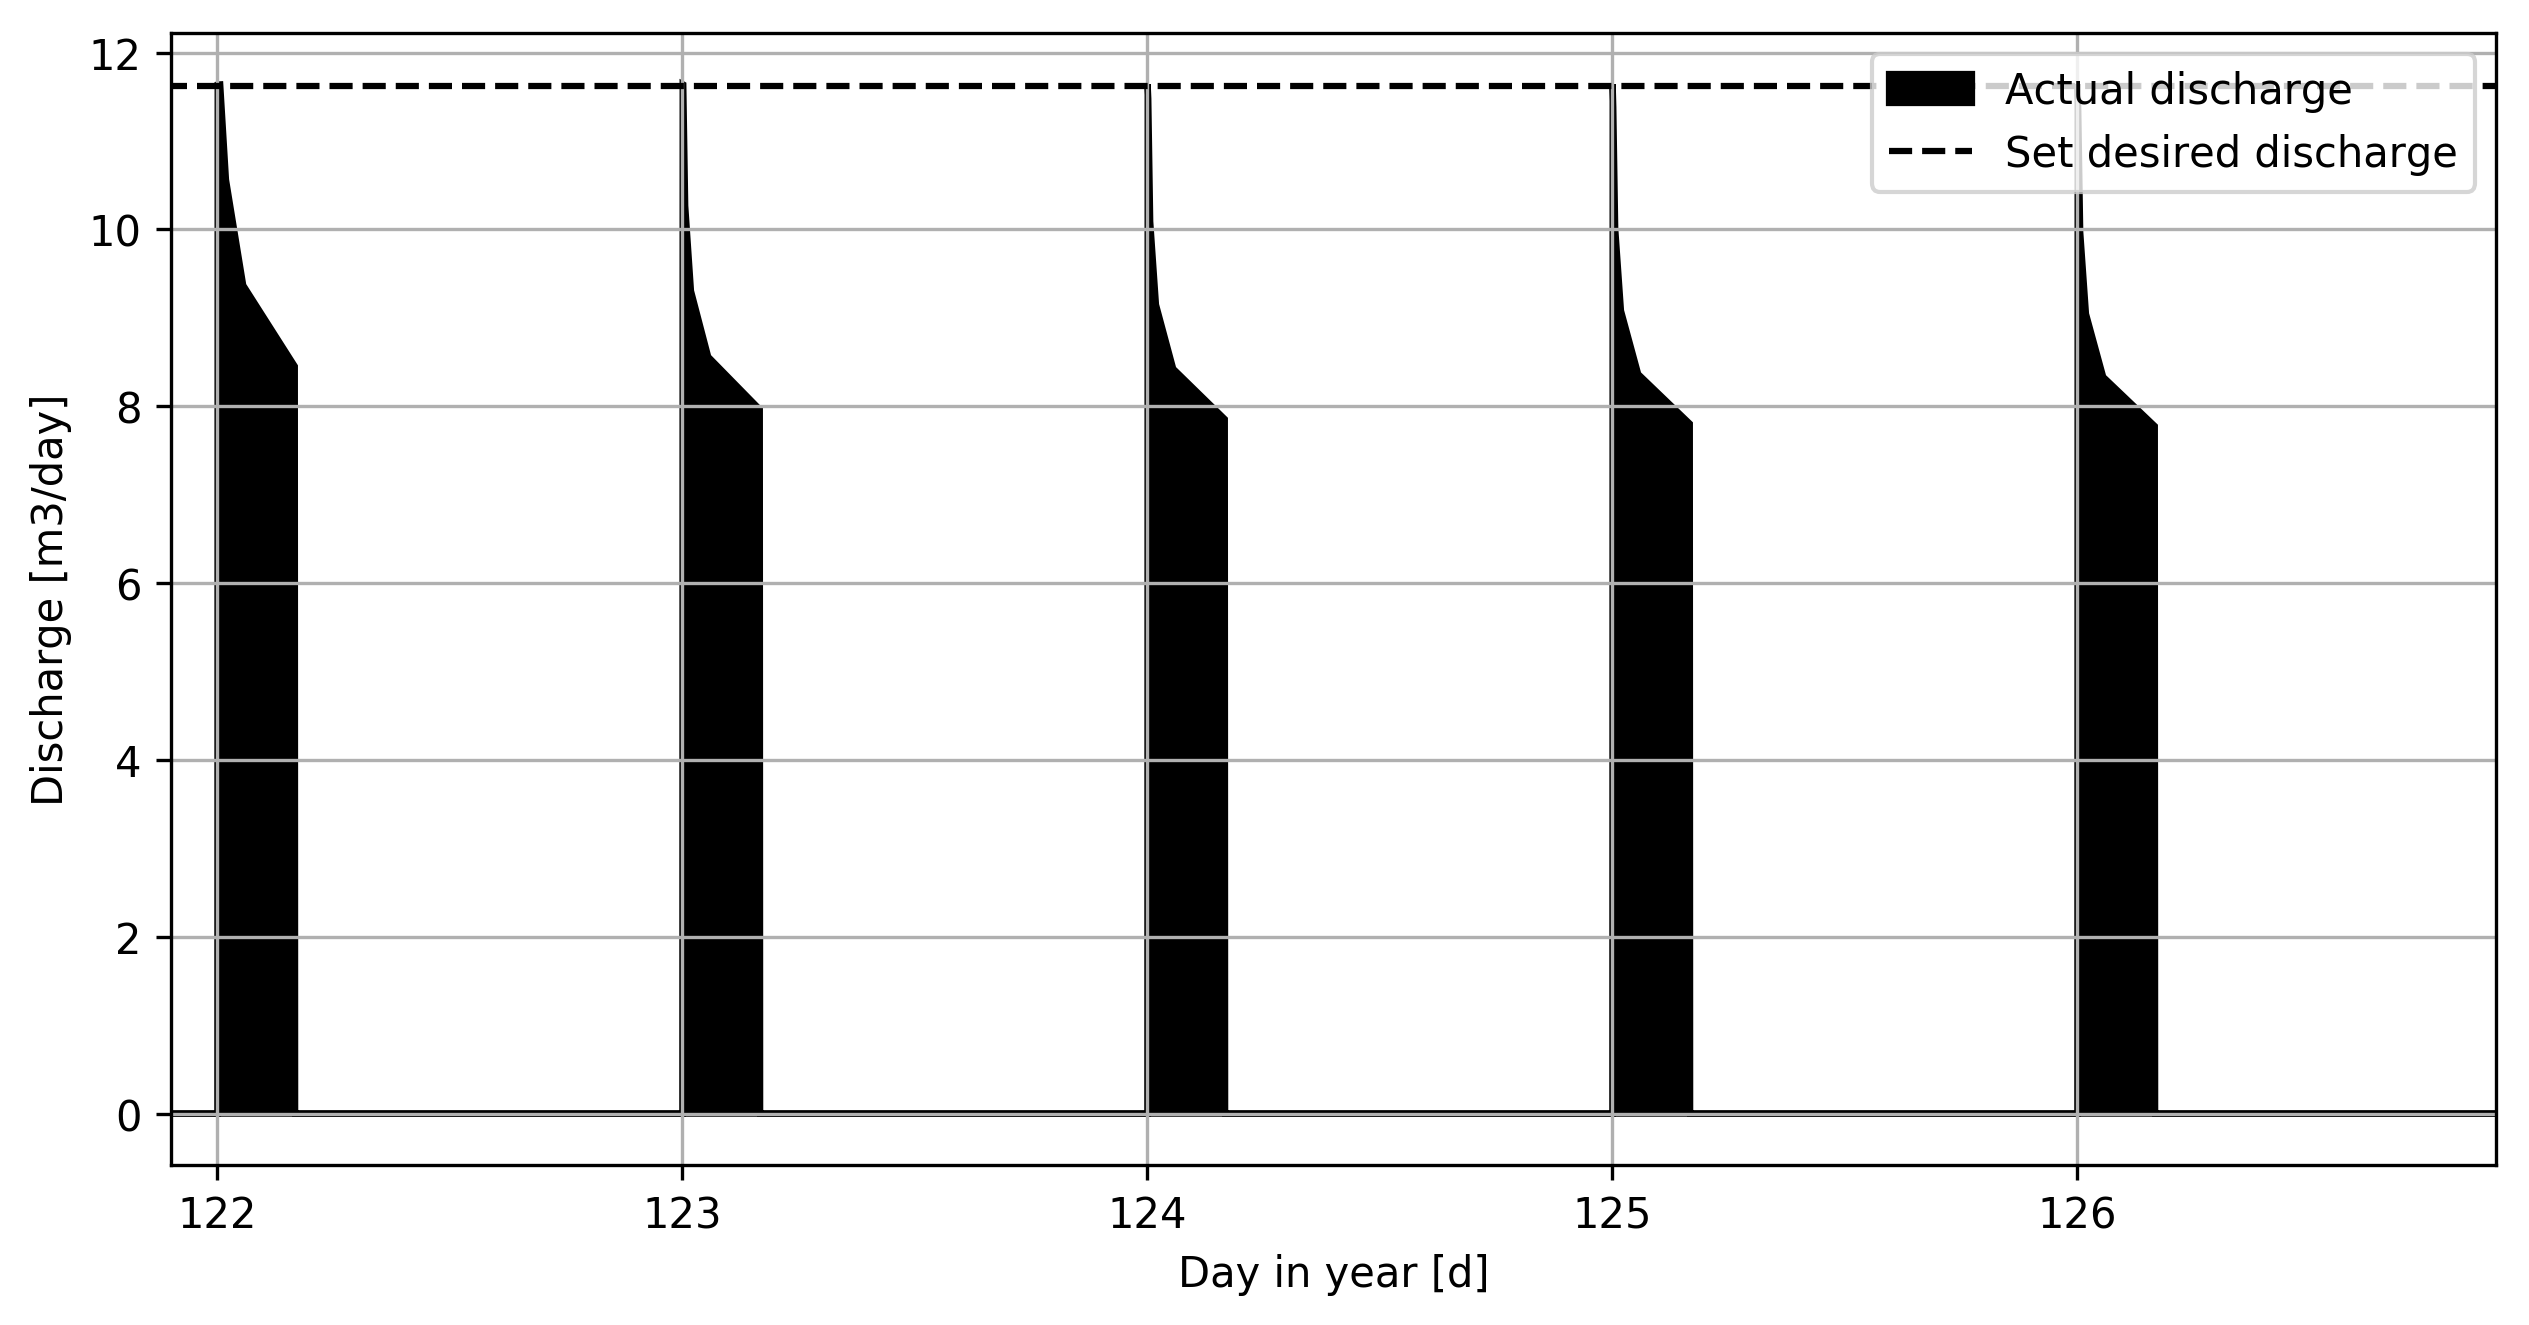
\includegraphics[width=\linewidth]{Sc1a5_Q122_126}
		\captionsetup{justification=centering}		
		\caption{\label{fig:Sc1a5_Q122_126}}
		\end{subfigure}\hfill
	\begin{subfigure}[b]{0.5\linewidth}
        \centering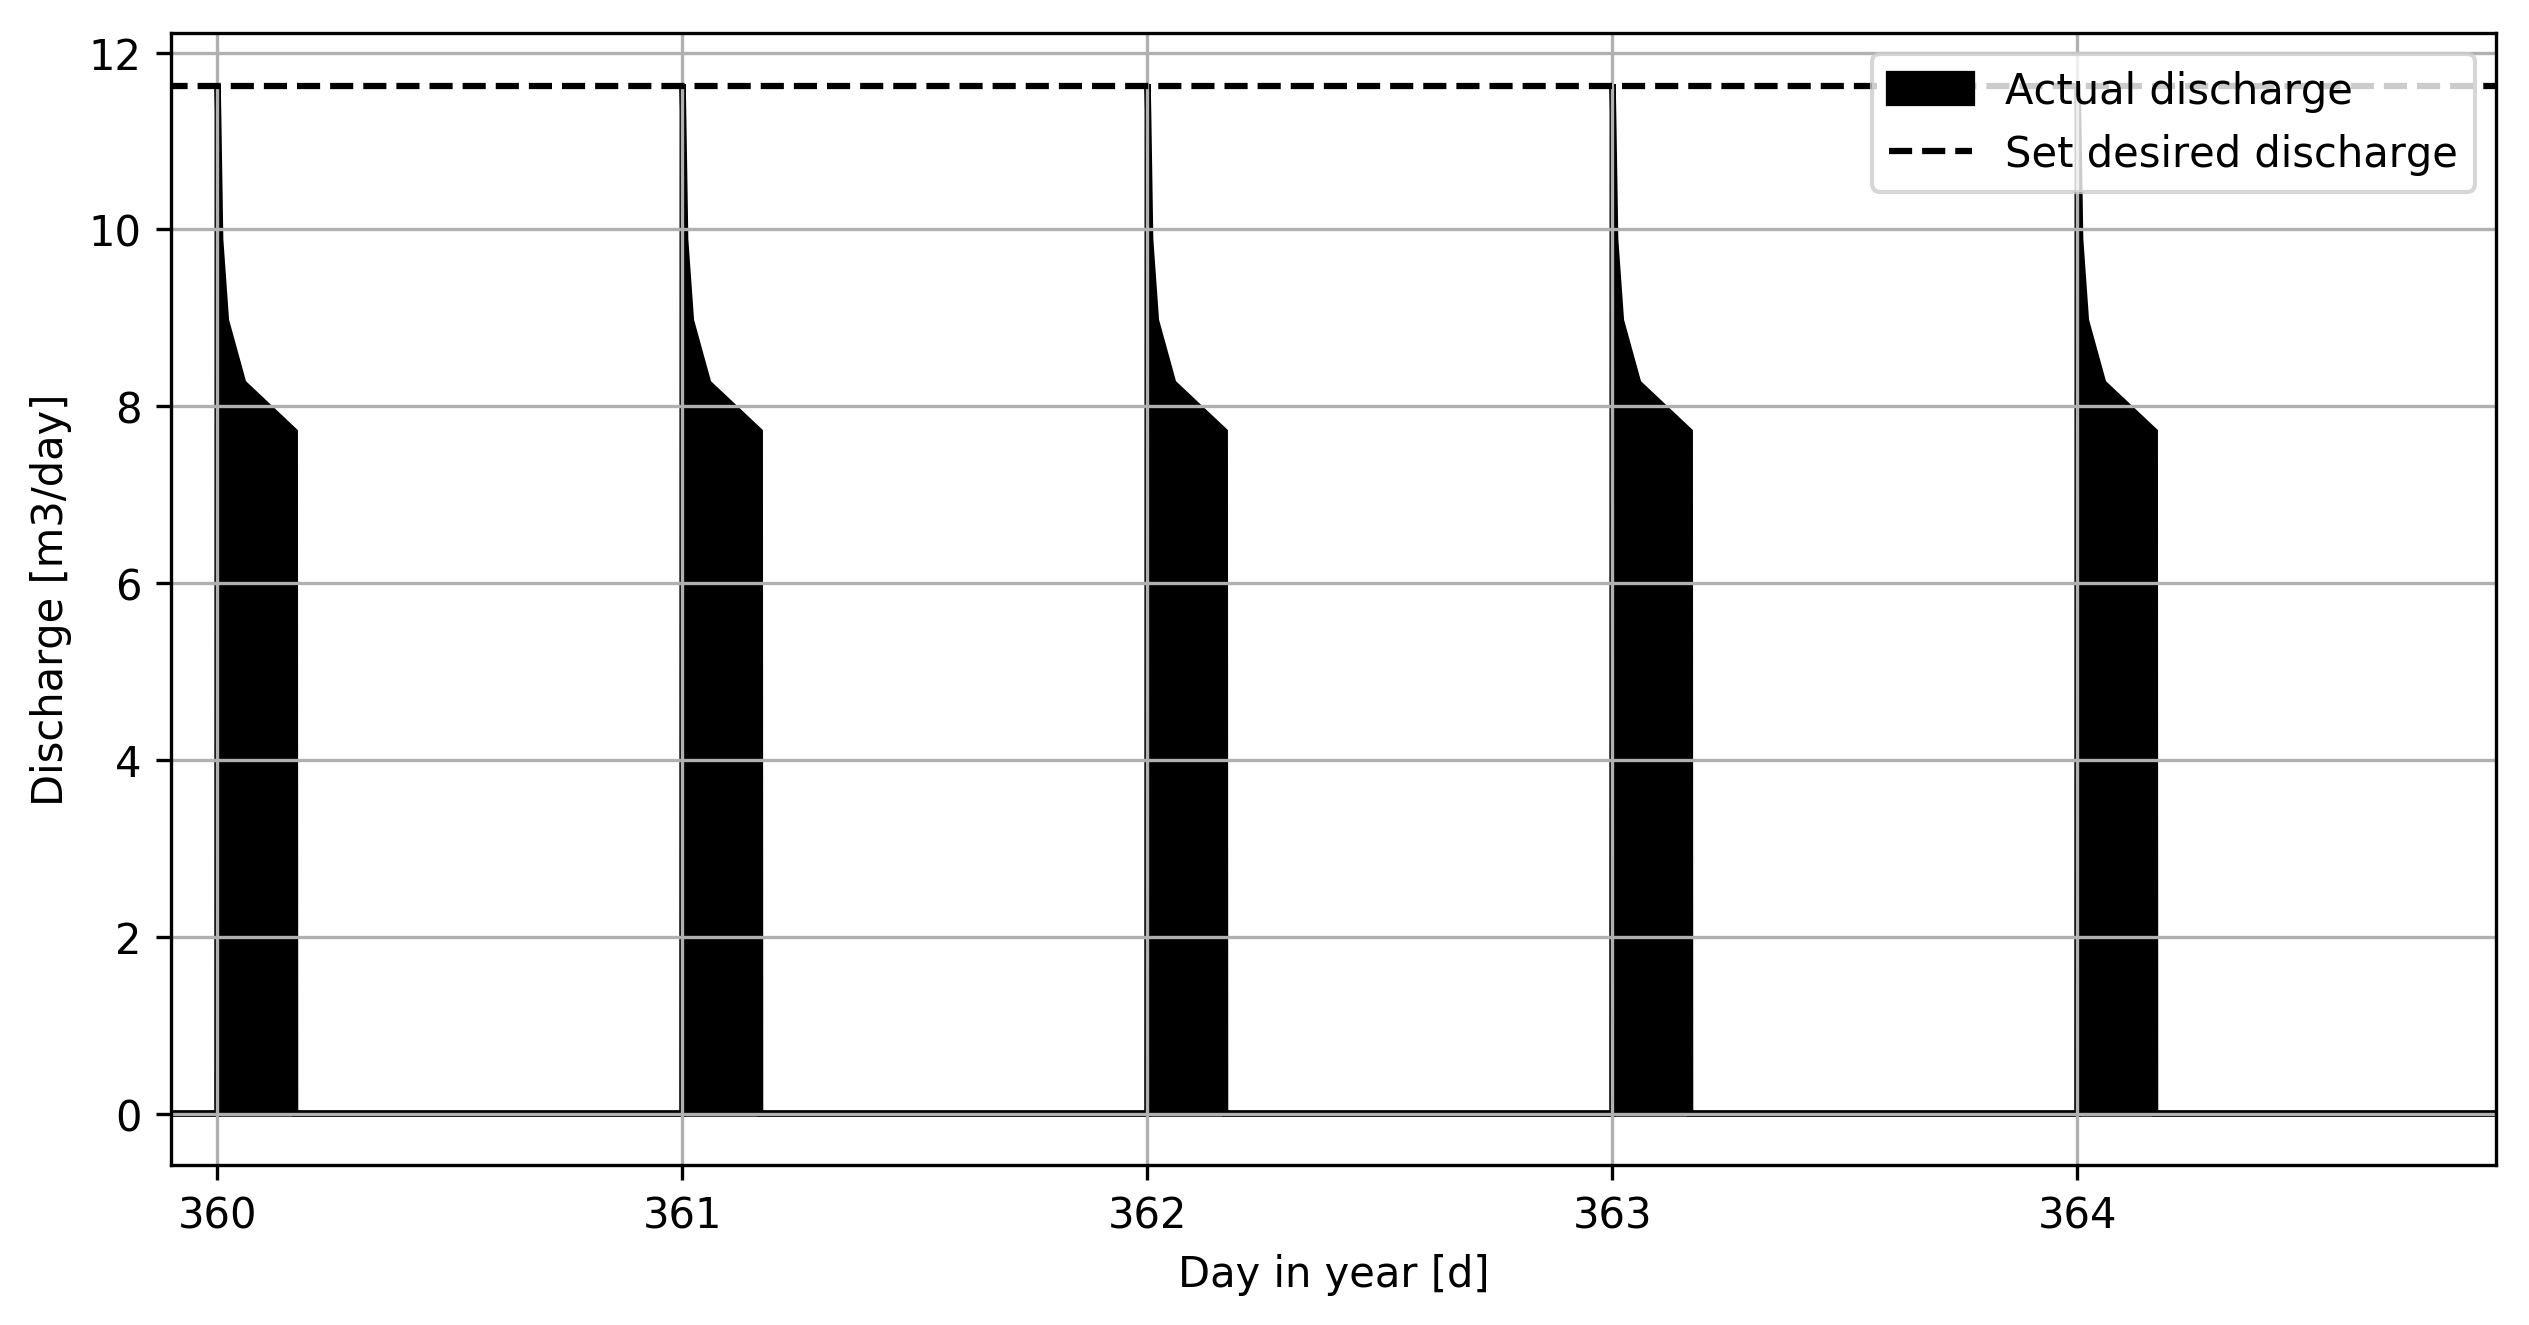
\includegraphics[width=\linewidth]{Sc1a5_Q360_364}
		\captionsetup{justification=centering}		
		\caption{\label{fig:Sc1a5_Q360_364}}
		\end{subfigure}
		\captionsetup{justification=centering}	
	\caption{Example scenario 1 - 5x base model well diameter - Discharge performance for (\subref{fig:Sc1a5_Q122_126}) the first five days and (\subref{fig:Sc1a5_Q360_364}) the last five days of dry season} 
	\label{fig:Example_Sc1_5x_diam_discharge}
\end{figure} 


\subsection{Upscaling by system cleaning}
\label{subsec:Up_clean}
Unlike the previous forms of upscaling, upscaling by system cleaning does not use the base model scenarios as reference start. All prior simulations are based on the assumption of a clean system. Fieldwork inspection showed clean systems are absent in nature. Debris accumulates at the borehole bottom. Direct consequence is a decrease in well penetration length. By the approach of a stepwise increase (5 steps) in borehole depth, the cleaning of a clogged borehole is simulated (\ref{fig:Schematic_up_clean}).   

\begin{figure}[H]
\centering
\begin{tikzpicture}
\node [mybox] (box){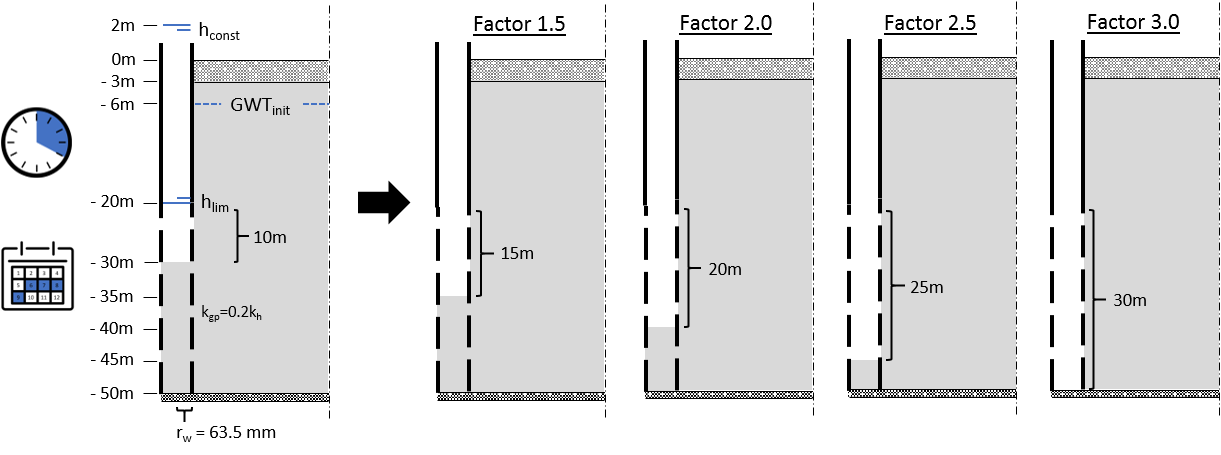
\includegraphics[width=0.9\linewidth]{Schematic_up_clean}};  
\node[title, right=10pt] at (box.north west) {Schematic upscaling well cleaning};
\end{tikzpicture}
\captionsetup{justification=centering}
\caption{Schematic upscaling penetration length due to well cleaning}
\label{fig:Schematic_up_clean}
\end{figure}

System cleaning has a positive impact on both the wet season recharge and dry season discharge. Total volumes infiltrated and withdrawn are approximately linear dependent on the (clean) well screen length. Effects of non-uniform flow (partially aguifer penetration) are not of significance for the simulation conditions applied in this study.  

\begin{figure}[h!]
 \centering
 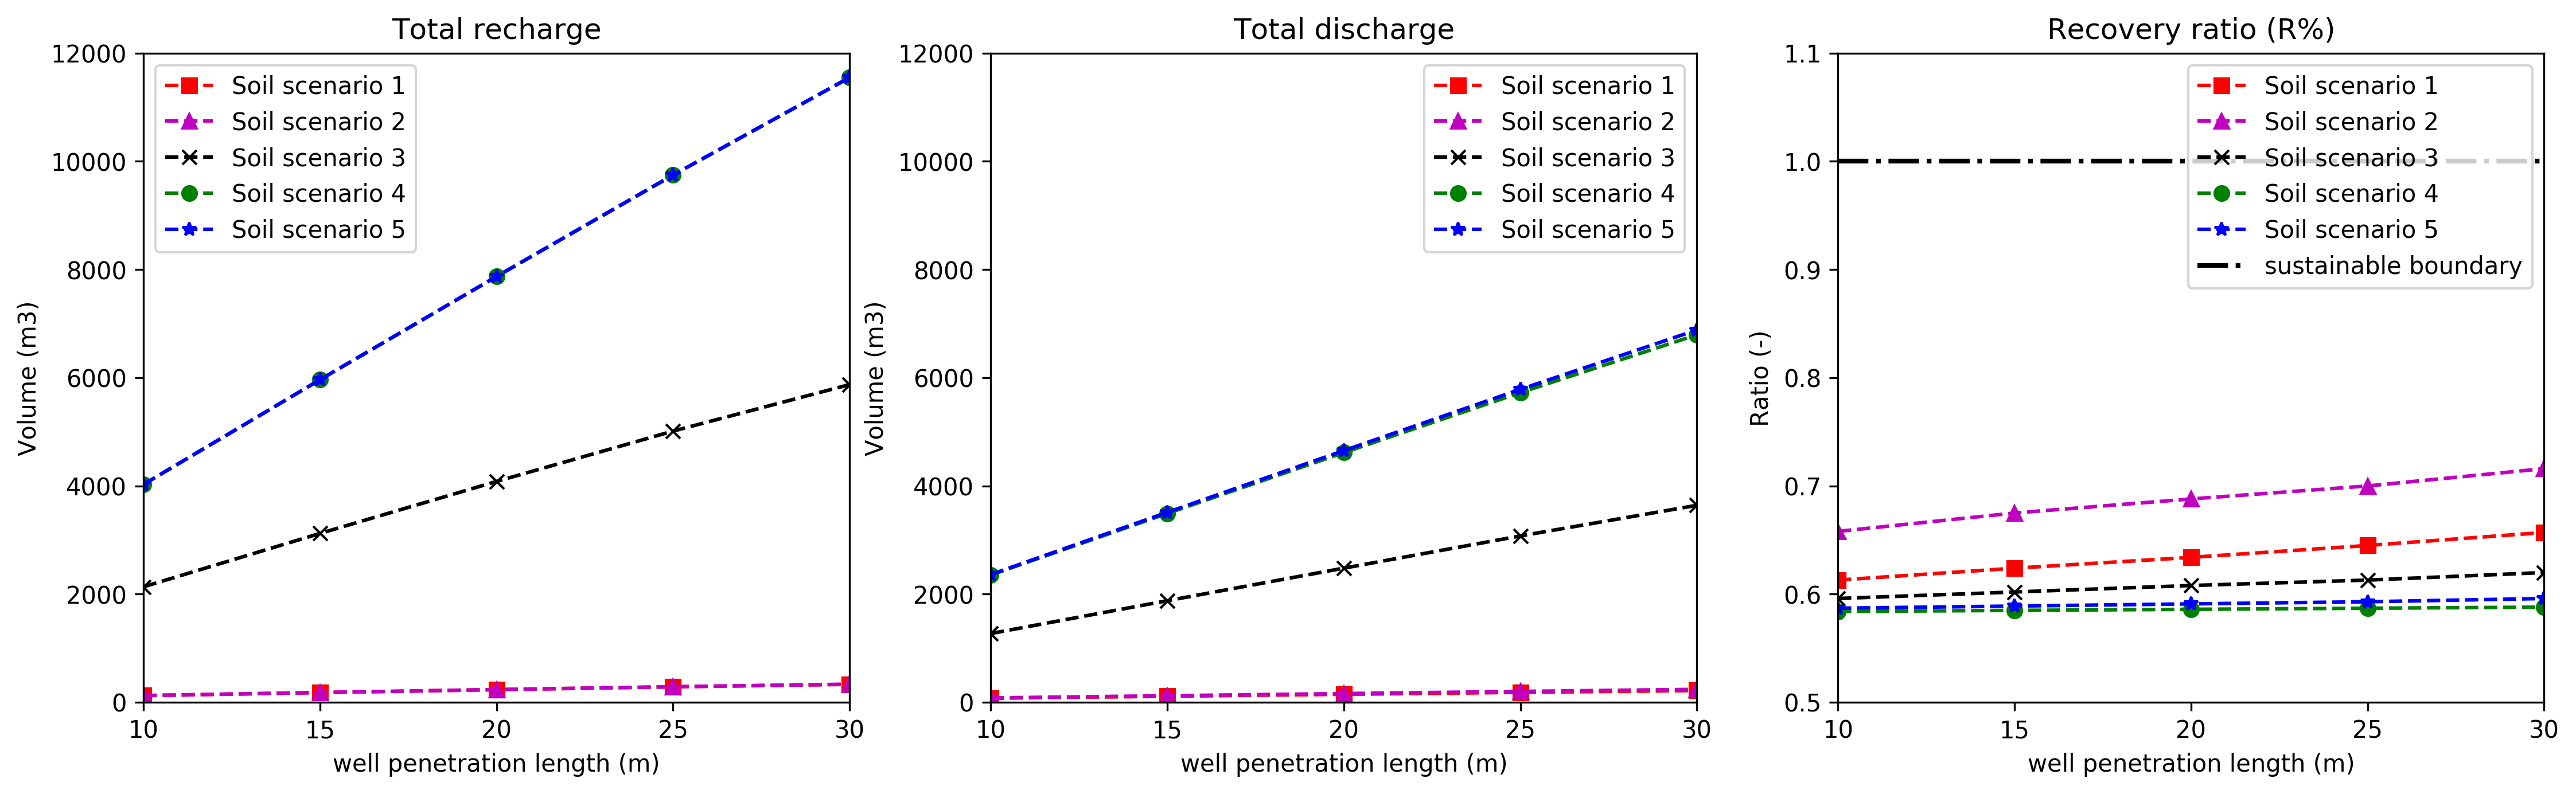
\includegraphics[width=1.0\linewidth]{Results_up_clean}
 \captionsetup{justification=centering} 
 \caption{Results of yearly total volumes (in, out, ratio) by upscaling the penetration length due to well cleaning}
 \label{fig:Results_up_clean}
\end{figure}

System cleaning ensures a increase in recovery ratios (for all soil scenarios). In an absolute sense the total volumes discharged are slightly more affected by cleaning compared to recharged volumes. In general recovery ratio increase is not significant. Moreover the ratios stay within the range of sustainable use. Deepening the borehole (to its original length) improves system operation. Cleaning of (partially) clogged systems is advisable. 

\section{Results \& Conclusions}
\label{section:Upscaling_conclusions}
brief conclusion on model simulation ASR-system performances are stated below: 
\begin{itemize}
\item{Base model scenarios} \\
In eight months of daily (4 hours) pump operation it is not possible to fully recover the volumes infiltrated due to four months of constant inundation (2 meter) on top of a well. Under the defined conditions of system composition and use, recovery ratios suggest a sustainable system impact on nature. 
\item{Upscaling daily pumping time}\\
Discharge volumes obtained by upscaling daily pump duration for the total eight months of dry season exceed the four months (gravity based) recharge volumes. Potential negative effects on nature (unsustainable system use) should be considered.
\item{Upscaling borehole cross-sectional dimension}\\
Magnification of the borehole diameter is beneficial for both groundwater recharge and discharge. Due to the non-linear relation, there is an upper limit in performance by further well enlargement.  
\item{Upscaling by system cleaning}\\
Deepening the borehole (to its original length) improves system operation. Cleaning of (partially) clogged systems is advisable. 
\end{itemize}

Further research can be pointed at a variety of topics:
\begin{itemize}
\item{\texttt{MNW2} skin resistance}\\
Little is known about the exact order of skin resistances (well conductance). A topic that can fill an entire individual research. It is for example unknown how to interpret the \texttt{CWC} in relation to a radial scaled MODFLOW model. Moreover, research can also be performed by the inclusion of a laboratory or fieldwork set-up. When fieldwork is done, a combination with infiltration bed resistances is possible. 
\item{additional options in ASR-system research}\\
Simulation are done by a constant flood bound of 2 m for four months. It would be interesting to investigate the ASR-system behaviour under the conditions of temporal flooding (rain-based inundation). 
\item{focus from water to crop}\\
crop required water withdrawel (potentially in combination with temporal storage in poly tank(s)). 
\item{sensitivity analysis}\\
A control sample should be applied on the model assumptions made. One can think of a sensitivy analysis regarding variation in constant head due to flooding, initial groundwater conditions, well skin resistances and/or set drawdown limitations. 
\end{itemize}